% This must be in the first 5 lines to tell arXiv to use pdfLaTeX, which is strongly recommended.
\pdfoutput=1
% In particular, the hyperref package requires pdfLaTeX in order to break URLs across lines.

\documentclass[11pt]{article}

% Remove the "review" option to generate the final version.
\usepackage[review]{EMNLP2023}
\usepackage{multirow}
% Standard package includes d   
\usepackage{times}
\usepackage{latexsym}
\usepackage{ulem}
% \usepackage{ctex}
% For proper rendering and hyphenation of words containing Latin characters (including in bib files)
\usepackage[T1]{fontenc}
% For Vietnamese characters
% \usepackage[T5]{fontenc}
% See https://www.latex-project.org/help/documentation/encguide.pdf for other character sets

% This assumes your files are encoded as UTF8
\usepackage[utf8]{inputenc}
\usepackage{url}
% This is not strictly necessary and may be commented out.
% However, it will improve the layout of the manuscript,
% and will typically save some space.
\usepackage{microtype}

% This is also not strictly necessary and may be commented out.
% However, it will improve the aesthetics of text in
% the typewriter font.
\usepackage{inconsolata}
\usepackage{graphicx}
\usepackage{framed}
\usepackage{array}
% for subfigure
\usepackage{subcaption}
\usepackage{CJK}
\usepackage{makecell}
\usepackage[most]{tcolorbox}
\usepackage{cleveref} 
\usepackage{pifont}
% \usepackage[cmyk]{xcolor}
\newcommand{\Blue}[1]{\colorbox[RGB]{153,204,255}{#1}}
\newcommand{\Yellow}[1]{\colorbox{yellow}{#1}}
\newcommand{\Green}[1]{\textcolor[RGB]{76,153,50}{#1}}
\newcommand{\Pink}[1]{\textcolor[RGB]{210,18,150}{#1}}
\newcommand{\secref}[1]{Sec. \ref{#1}}
\newcommand{\figref}[1]{Figure \ref{#1}}
\newcommand{\eqnref}[1]{Eq. (\ref{#1})}
\newcommand{\tabref}[1]{Table \ref{#1}}
\newcommand{\exref}[1]{Example \ref{#1}}

\newcommand{\KZ}[1]{\textcolor{blue}{(Kenny: #1})}
\newcommand{\MY}[1]{\textcolor{red}{(Mengyue: #1})}
\definecolor{shadecolor}{RGB}{224, 224, 224}
\definecolor{framecolor}{RGB}{160,160,160}
% \definecolor{shadecolor}{RGB}{241, 241, 255}
% \newenvironment{prompt}
% {\begin{center}\begin{minipage}{0.9\linewidth}\begin{shaded} \small}
% {\end{shaded}\end{minipage}\end{center}\par}
\newenvironment{prompt}
{\begin{center}\begin{tcolorbox}[colback=shadecolor,%gray background
                  colframe=framecolor,% black frame colour
                  width=7.4cm,% Use 8cm total width,
                  arc=2mm, auto outer arc,
                  boxrule=0.3pt,
                 ] \small}
{\end{tcolorbox}\end{center}\par}


% If the title and author information does not fit in the area allocated, uncomment the following
%
%\setlength\titlebox{<dim>}
%
% and set <dim> to something 5cm or larger.

% \title{Leveraging ChatGPT to Power Chatbots for Psychiatric Diagnosis and Patient Simulation}
\title{LLM-empowered Chatbots for Depression Diagnosis: \\Simulation and Evaluation}
% \title{Realistic Simulation Doctor and Patients for Psychiatric Diagnosis}

% Author information can be set in various styles:
% For several authors from the same institution:
% \author{Author 1 \and ... \and Author n \\
%         Address line \\ ... \\ Address line}
% if the names do not fit well on one line use
%         Author 1 \\ {\bf Author 2} \\ ... \\ {\bf Author n} \\
% For authors from different institutions:
% \author{Author 1 \\ Address line \\  ... \\ Address line
%         \And  ... \And
%         Author n \\ Address line \\ ... \\ Address line}
% To start a separate ``row'' of authors use \AND, as in
% \author{Author 1 \\ Address line \\  ... \\ Address line
%         \AND
%         Author 2 \\ Address line \\ ... \\ Address line \And
%         Author 3 \\ Address line \\ ... \\ Address line}

\author{Siyuan Chen$^1$, Mengyue Wu$^2$\thanks{~~Corresponding Authors.}, Kenny Q. Zhu$^{3*}$,  \\ 
{\bf Kunyao Lan$^4$}, {\bf Zhiling Zhang$^5$}, {\bf Lyuchun Cui$^6$} \\
$^{1,2,3,4,5}$Shanghai Jiao Tong University, Shanghai, China \\
$^{6}$Shanghai Mental Health Center, Shanghai, China \\
\texttt{\{$^1$chensiyuan925, $^2$mengyuewu, $^4$lankunyao, $^5$blmoistawinde\}@sjtu.edu.cn,}\\
\texttt{$^3$kzhu@cs.sjtu.edu.cn, $^6$cuilvchun@outlook.com}
}


  % Affiliation / Address line 1 \\
  % Affiliation / Address line 2 \\
  % Affiliation / Address line 3 \\
  % \texttt{email@domain} \\\And
  % Second Author \\
  % Affiliation / Address line 1 \\
  % Affiliation / Address line 2 \\
  % Affiliation / Address line 3 \\
  % \texttt{email@domain} \\}

% \author{Siyuan Chen \and Mengyue Wu\thanks{~~Corresponding Authors.} \\ \and {\bf Kunyao Lan} \and {\bf Zhiling Zhang} \\ \and {\bf Minghao Lyu} \and {\bf Kenny Q. Zhu$^*$ } \\
% Shanghai Jiao Tong University \\
% Shanghai, China \\
% \texttt{\{chensiyuan925, mengyuewu, lankunyao, blmoistawinde\}@sjtu.edu.cn,}\\ 
% \texttt{qianlan844@gmail.com, kzhu@cs.sjtu.edu.cn}\\ 
% \And Lyuchun Cui \\
% Shanghai Mental Health Center\\
% Shanghai, China\\
% \texttt{cuilvchun@outlook.com}
% }


\begin{document}
\maketitle
\begin{abstract}
While using chatbots in mental health domain is receiving increasing amount of attention, implementation and evaluation of chatbots in psychiatric diagnostic scenarios remains relatively unexplored.
In this work, we focus on exploring the potential of ChatGPT in powering chatbots to simulate psychiatrist and patient for depression diagnosis. 
We collaborate with professionals to identify key objectives of such bots and iteratively develop the dialogue system to closely align with real-world scenarios. 
Additionally, we design task-specific evaluation metrics, and involve real psychiatrists and patients in diagnostic conversations with the chatbots, collecting their ratings for assessment.
Experiments shows that our doctor chatbot exhibits higher levels of empathy and diagnostic accuracy compared to the baseline; our patient chatbot can replicate human-like behaviors, including emotional fluctuations.

% \KZ{If outpatient scenarios are under-explored, then in-patient has been well studied? Shall we just say diagnotic vs.  therapeutic scenarios?}\MY{check all other  places you use``outpatient'', some can be changed into diagnostic some can just use clinical}
\end{abstract}
% COMMENT: 摘要中是不是可以简单提一下机器人诊断和模拟病人的科研或实用价值


\section{Introduction}
\label{sec:intro}

There is a growing interest in applying conversational agents (i.e., chatbots) in the mental health domain~\cite{sabour2022chatbots}. Chatbots that can (i) conduct diagnosis conversations like a psychiatrist or (ii) simulate patients in the psychiatric diagnostic scenarios, have significant real-world applications\footnote{For the sake of clarity, we will refer to these two types of chatbots as the \textbf{``doctor chatbot''} and \textbf{``patient chatbot''} respectively in the subsequent sections.}. 
Doctor chatbots can be effective tools for mental disorder screening~\cite{pacheco2021Smart} in lieu of official medical diagnosis. Patient chatbots can serve as Standard Patients (SP) in medical education, making the learning process more efficient and cost-effective~\cite{Torous2021growing}.

However, there is still limited exploration in developing and evaluating these 
chatbots, primarily due to the difficulty in obtaining dialogue data because 
of the ethical and privacy concerns for mental health issues. 
% \KZ{you just said earlier that conversational agents are increasingly being used in mental health, but now you say limited exploration. Contradictory?} 
What's more, in outpatient scenarios, depressed patients often find it difficult 
to describe their ambiguous mental state objectively, 
and they may even be ashamed or afraid of disclosing their true 
conditions~\cite{Salaheddine2016Identify}. As a result, doctor chatbots should 
go beyond serving as interactive scales (e.g., PHQ-9) for mental disorder 
screening~\cite{Yue2023Beyond}. They need to possess various professional 
skills, including emotional support, to effectively complete the diagnosis task.
Additionally, patient chatbots should resemble real patients more closely, 
rather than precisely and robotically reporting their symptoms without 
any emotional fluctuations.

\begin{figure*}[th]
	\centering
	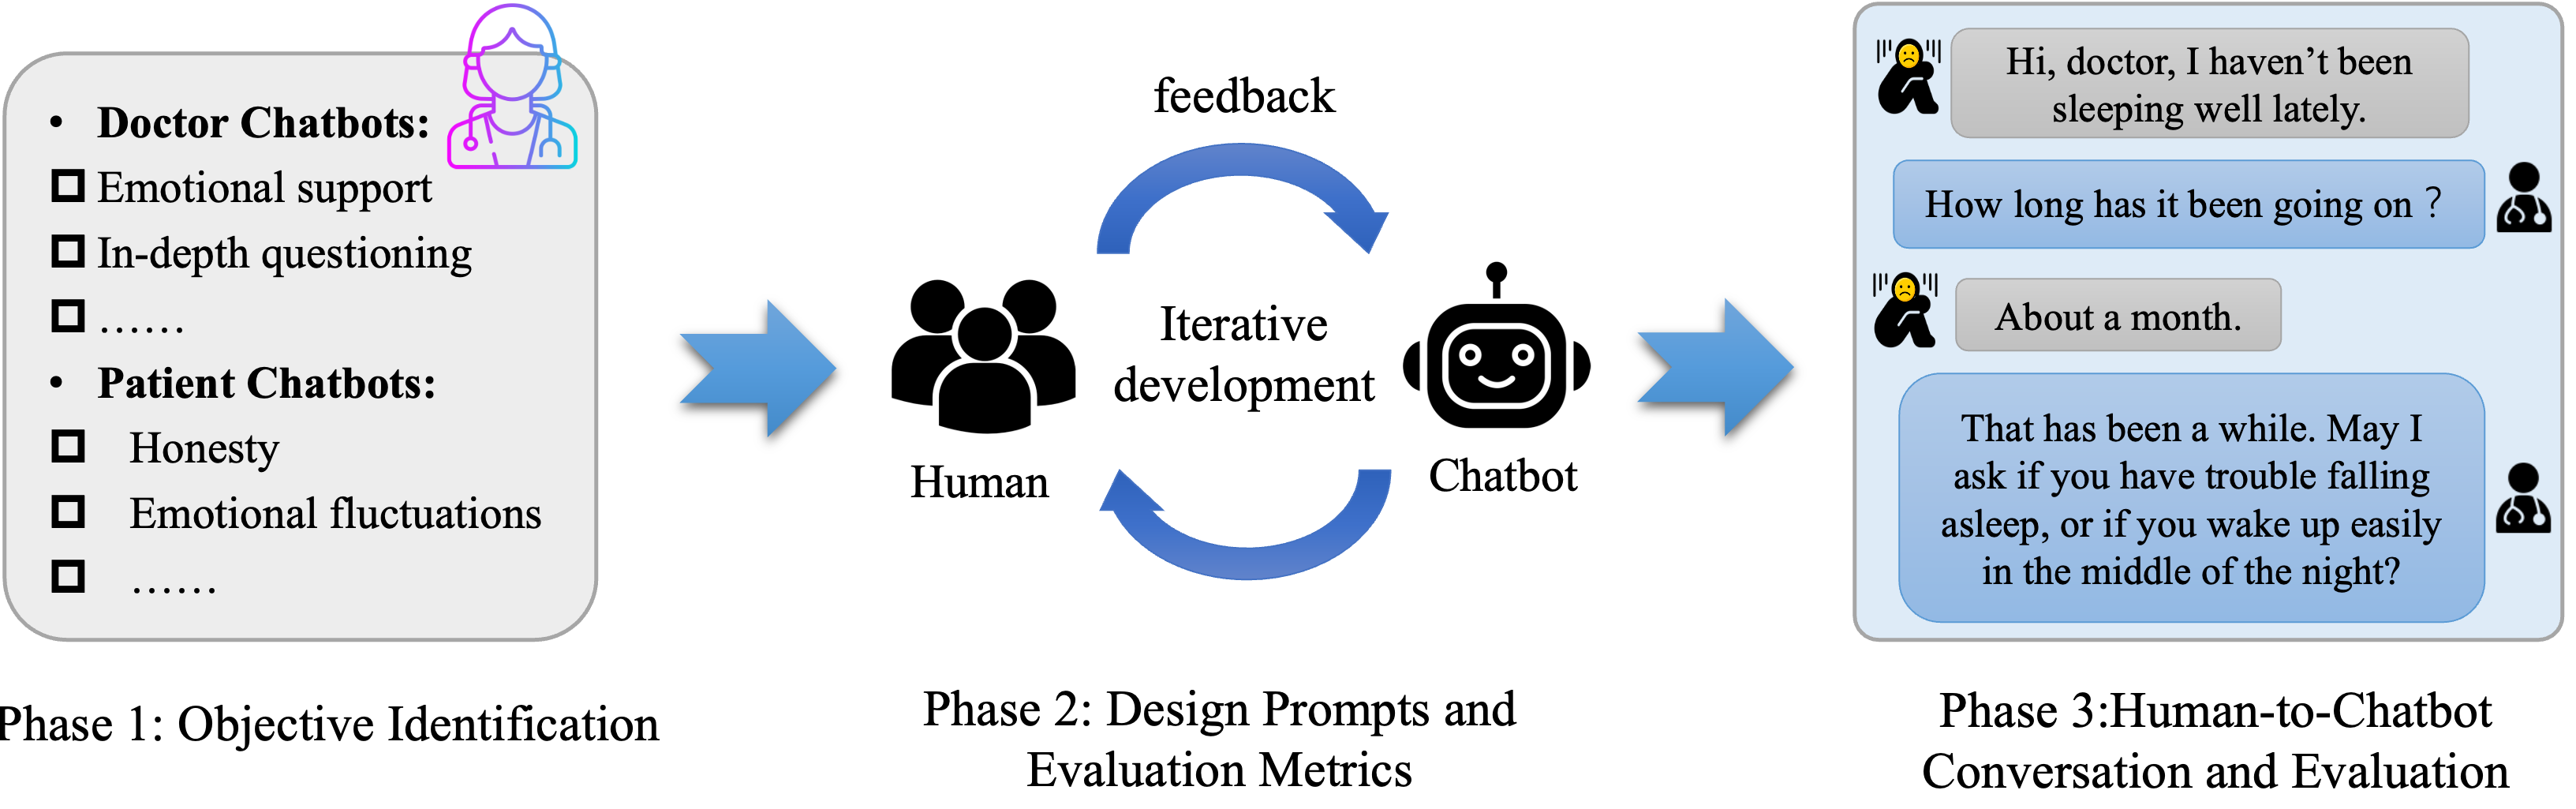
\includegraphics[width=0.8\linewidth]{Figures/overview.png}
	\caption{The overview of the expert-guided three-phase study.}
	\label{fig:pipeline}
\end{figure*}

% However, many existing frameworks~\cite{Medeiros2018UsingCF,Jaiswal2019Virtual} still rely on rule-based approaches (e.g., utilize the questions in self-rating scales), which often result in rigid conversations and cannot show sufficient empathy to patients. Alternatively, other deep learning methods \cite{yao-etal-2022-d4} require a significant amount of domain-specific data for training, which is often costly and difficult to obtain, especially in the mental health domain. 
% Furthermore, due to the diverse ways to express mental states verbally, neither rule-based nor data-based methods can comprehensively cover all possible cases, so the patient chatbots developed using these methods tend to be inflexible and lack diversity~\cite{Yao2020Toward}.

% \KZ{But how is simulating doctors and patient in diagnosis conversation more difficult than the therapeutic bots in Woebot and Wysa, and the like? In other words, why can't we use the techniques in Woebot and Wysa to simulate doctors and patients? I think the difference between diagnostic bots and therapeuric bots is that it's easier to verify quality of the doctor bot or patient bot: a good doctor bot must be able to acquire enough info efficiently from the patient so as to make a correct diagnosis; a good patient bot must resemble the real patient in doctors eyes. A good therapist however can't be easily qualified because all they are doing is to make the patient feel better, which is very subjective from the patient point of view.}  


Achieving these goals is quite difficult for conventional rule-based~\cite{Medeiros2018UsingCF,Jaiswal2019Virtual} or even data-driven~\cite{yao-etal-2022-d4, Fansi2022DDXPlus, Lin2021Graph} methods. This difficulty arises from the complexity of understanding varied human utterance in diagnosis conversations with a limited amount of pre-defined rules or training data. 
% \MY{Any reason why data-drive is not enough as well?} 
Fortunately, recent advancements in large language models (LLMs), such as ChatGPT\footnote{\url{https://chat.openai.com/}}, provide a new way to develop chatbots that can convincingly portray specific roles for its superior capability in understanding diverse natural language~\cite{Pan2023APE} and generating coherent conversations. Importantly, LLMs can achieve this with appropriate prompts rather than fine-tuning on extensive domain data.

% Equipped with comprehensive training data and knowledge, LLMs can generate diverse tones and symptom descriptions with appropriate prompts rather than fine-tuning on extensive domain data.\MY{what i meant is that why LLM can do it is not only because of its strength in generation but also understanding, these should be aligned with the challenges when using data-drive approaches}


% Achieving these goals is quite difficult for conventional rule-based~\cite{Medeiros2018UsingCF,Jaiswal2019Virtual} or even data-driven~\cite{yao-etal-2022-d4, Fansi2022DDXPlus, Lin2021Graph} methods, due to the difficulty of adequately covering complex cases of psychiatric diagnosis with a limited amount of pre-defined rules or training data. 
% % \MY{Any reason why data-drive is not enough as well?} 
% Fortunately, recent advancements in large language models (LLMs), such as ChatGPT\footnote{\url{https://chat.openai.com/}}, provide a new way to develop chatbots that can convincingly portray specific roles\MY{for its superior capability in understanding diversed natural language and generating coherant coversations, better add a ref}.  Equipped with comprehensive training data and knowledge, LLMs can generate diverse tones and symptom descriptions with appropriate prompts rather than fine-tuning on extensive domain data.\MY{what i meant is that why LLM can do it is not only because of its strength in generation but also understanding, these should be aligned with the challenges when using data-drive approaches}

% COMMENT: 前面所述,该chatbot的困难有两点:数据难采集和症状的模糊、主观。这里只讲清楚了ChatGPT能够解决数据采集的问题,那么它怎么来应对症状模糊主观的问题呢?此外还包括刚才上一段提到的,diagnosis chatbot需要提供情感支撑,patient simulator要仿真病人的情绪波动,要如何实现,这里是不是都应该简单描述一下?

Therefore, in this work, we aim to (i) respectively investigate the potential of ChatGPT in simulating \textit{psychiatrists} and depressed \textit{patients} in a clinical diagnosis scenario, 
as well as to (ii) build a comprehensive evaluation framework for these chatbots, answering the question about what constitutes a good psychiatrist chatbot and a truly patient-like chatbot.

To develop and evaluate a system that truly meets the the user's expectations, 
we follow a expert-guided design methodology. The study consists of three 
phases (See Figure~\ref{fig:pipeline}).
In \textbf{Phase 1}, as there lacks a formal description of the objectives for 
doctor and patient chatbots, we first collaborate with psychiatrists to 
identify them clearly. 
Based on these objectives, we conduct an experimental study 
(\textbf{Phase 2}) to design appropriate prompts for ChatGPT-based chatbots 
and establish an evaluation framework that incorporates both human evaluation 
and automatic evaluations aligned with the objectives from Phase 1. Importantly, the design of prompts and metrics was iterated based on human feedback, with each version improved with input from psychiatrists.
In \textbf{Phase 3}, we recruit real psychiatrists and depression patients to 
engage in diagnostic conversations with the 
simulated patient and doctor chatbots, respectively, and collect their 
ratings after conversation.
% We also conduct a comparison between the behavior of real and simulated psychiatrists based on the dialogue history, which yields some interesting findings. 

The main contributions of this work are:
\begin{itemize}
    \item We formalize the task of developing doctor and patient chatbots for depression diagnosis within an outpatient setting. In doing so, we propose specific \textit{objectives} for these chatbots that are up to near-clinical standards and establish an \textit{evaluation framework} that aligns with these objectives, with the help of practicing psychiatrists.
    \item We adopt an iterative prompt engineering approach, taking into account psychiatrists' feedback to refine the performance. By utilizing \textit{examples}, we enhance ChatGPT's understanding of professional practices. We further implement a \textit{reminder} mechanism to mitigate potential issues of forgetting when the desired behavior of chatbot being different from LLM's training purpose.
    % \MY{why is forgetting so common in our application, if it is a general phenomenon, we might want to change the reminder as patient behaviour being different from LLM's training purpose}
    \item We demonstrate the feasibility of utilizing ChatGPT-powered chatbots in mental health domain. Experiments show that ChatGPT-based doctor chatbot provides more accurate diagnostic results through more empathetic and efficient conversations with patients, comparing to the previous machine-learned chatbots.
    % \KZ{This is the first time you mention ``data-driven chatbot''. What exactly is it? Are you referring to CPT only?} 
    Moreover, the patient chatbot also exhibits emotional expression and 
resistance, which is similar to real patients. 
    % \item We suggest a data augmentation strategy that employs carefully evaluated doctor and patient chatbots to produce unlimited psychiatric outpatient dialogue data, effectively tackling the obstacle of obtaining data due to ethical concerns in mental health domain. We also provide the dataset containing dialogues between chatbots and real patients or psychiatrists from our evaluation experiments, which has been anonymized for privacy. 
    % \KZ{Ethical and privacy concerns?}
\end{itemize}




% Intuitively, relying on traditional evaluation metrics for dialogue systems (e.g., n-gram overlap, semantic textual similarity) to assess the performance of doctor and patient chatbots in mental health scenarios is inadequate, as there is no standardized answer for clinical conversations. 
% Moreover, what constitutes an exceptional psychiatrist chatbot or a realistic patient chatbot still remains unexplored. 

% Applications designed for mental health therapy or coaching in daily life, such as Woebot\footnote{\url{https://woebothealth.com}} and Wysa\footnote{\url{https://www.wysa.com}}, are gaining widespread attention for their ability to reduce users' negative emotions~\cite{Grove2021Codevelop} and promote a healthy lifestyle~\cite{Fadhil2019AssistiveCA}. Another notable application is chatbot-based symptom checkers~\cite{Yue2023Beyond}, which emulate human-like conversations while assessing users' symptoms, resembling interactive questionnaires.


\section{Objectives}
% objectives
\label{sec:objectives}
% In this paper, we ask the following scientific question:
% \begin{quote}
%     ``What constitutes a realistic doctor/patient chatbot in psychiatric outpatient conversations?'' 
% \end{quote}

Given the lack of formal definition for what constitutes a good doctor/patient chatbot in psychiatric diagnosis conversations, we invite five experienced psychiatrists to establish clear objectives and standards, which will guide us throughout the study\footnote{These psychiatrists come from top-ranked national mental health centers. 
Their professional titles and areas of expertise can be found in 
Appendix \ref{apd:psych_info}.}. 
The objectives are derived from the first two phases. In phase 1, the psychiatrists are encouraged to freely express their opinions, allowing us to summarize a set of objectives.  In phase 2, as we iteratively refine the prompts, we consult the psychiatrists for their input and identify any additional objectives to consider based on the performance of chatbot. The final objectives are organized as follows.
% \MY{how do we know that at last stage, this is the final standard? do we have a comment from doctors that the defined objectives are exhaustive and up to application standard?}

% \KZ{The following is a bit weird. Shall we change our title to include depression? Since this paper focuses on bots to diagnose depression only?}
% Considering the variation in diagnosis standards and symptoms for different mental disorders, we concentrate on depressive disorders for this study, while leaving the scaling to include other disorders as future work.

\subsection{Doctor Chatbot}
\label{sec:doc_requirements}
As a doctor chatbot, the primary task is to conduct a professional diagnostic process for the patient and provide an \textbf{accurate diagnosis}. To achieve this, a good doctor chatbot should possess the following three capacities:
% \MY{I don't think empathy-related stuff is only for user experience, it also serves the purpose of building inter-personal relation and trust for the patients, and eased their nerves for the purpose of better revealing truthful feelings and symptoms, hence a more accurate diagnosis}
\begin{itemize}
    \item \textbf{Comprehensiveness:} Inquire about the key symptoms of depression, including sleep, mood, diet, and other relevant aspects that are required for diagnosis, as defined in DSM-5~\cite{american2013diagnostic}.
    \item \textbf{In-depth Questioning:} Conduct thorough questioning (e.g., ask the duration of a symptom) based on patient's responses to gain a more precise evaluation of the symptoms.
    \item \textbf{Empathy:} Demonstrate empathy and provide emotional support to patients to establish trust and ease their nerves. This helps patients feel more comfortable in expressing their genuine feelings and symptoms, leading to a more accurate diagnosis.
    % \item Provide examples to guide patients to articulate their symptoms, rather than just asking, "Do you have any other symptoms?", the latter often causing patients to overlook important symptoms and forget to mention to the doctor.
\end{itemize}
Moreover, to offer patients superior \textbf{user experience}, the doctor chatbot should fluently switch between topics and enhance the efficiency of the conversation, thus preventing patients from feeling bored or disengaged.
\subsection{Patient Chatbot}
\label{sec:pat_requirements}

% After establishing objectives for doctor chatbots, we encountered difficulties when defining the requirements for chatbots that resemble real patients. This is due to the fact that individuals with the same disorder can exhibit significant variations in their manifestations. Moreover, psychiatrists, though experienced, have no firsthand chatting experience with a ``non-patient-like'' chatbot, making it challenging for them to generalize the requirements for a ``patient-like'' chatbot.

% To address this issue, we decide to develop an initial version of the chatbot first. This allows psychiatrists to interact with ``non-patient-like'' examples, which can help them better define the characteristics and behaviors that constitute a ``patient-like'' chatbot. Based on their feedback, we then iterate and update the chatbot accordingly.
% At this phase, we only establish one fundamental requirement for a patient chatbot.

The basic requirement for a patient chatbot is \textbf{honesty}, which entails presenting an accurate and rational description of symptoms in the provided symptom list, without reporting any non-existent ones.

Additionally, to make the chatbot more resemble real patients, psychiatrists also describe some behaviors commonly exhibited by real patients during consultations. 
\begin{itemize}
    \item \textbf{Emotion:} Patients in a depressed mental state may experience emotional fluctuations during the conversation.
    % while the chatbot's presentation of symptoms is too calm and polite. 
    \item \textbf{Expression:} Patients use colloquial expressions when describing symptoms, and may have difficulty expressing themselves clearly. They often talk about their daily life experiences. While current chatbots tend to explicitly list out the symptoms~\cite{Llanos2021Lessons} using formal language, which is too sane and professional for a patient.
    % However, the chatbot tends to use formal language similar to the official diagnostic criteria (DSM-5).
    \item \textbf{Resistance:} Patients may be reluctant to seek help. They may remain silent and refuse to communicate, or downplay their symptoms to avoid being perceived as a burden. 
    % In contrast, the chatbot is overly cooperative, readily acknowledging and providing detailed descriptions of its symptoms.
\end{itemize}




% \section{Background and Related Work}
In this section, we present the necessary background knowledge about matrix factorization and unstructured pruning (\figref{fig:intro}).

\begin{figure}[t!]
	\centering
	\scalebox{0.154}{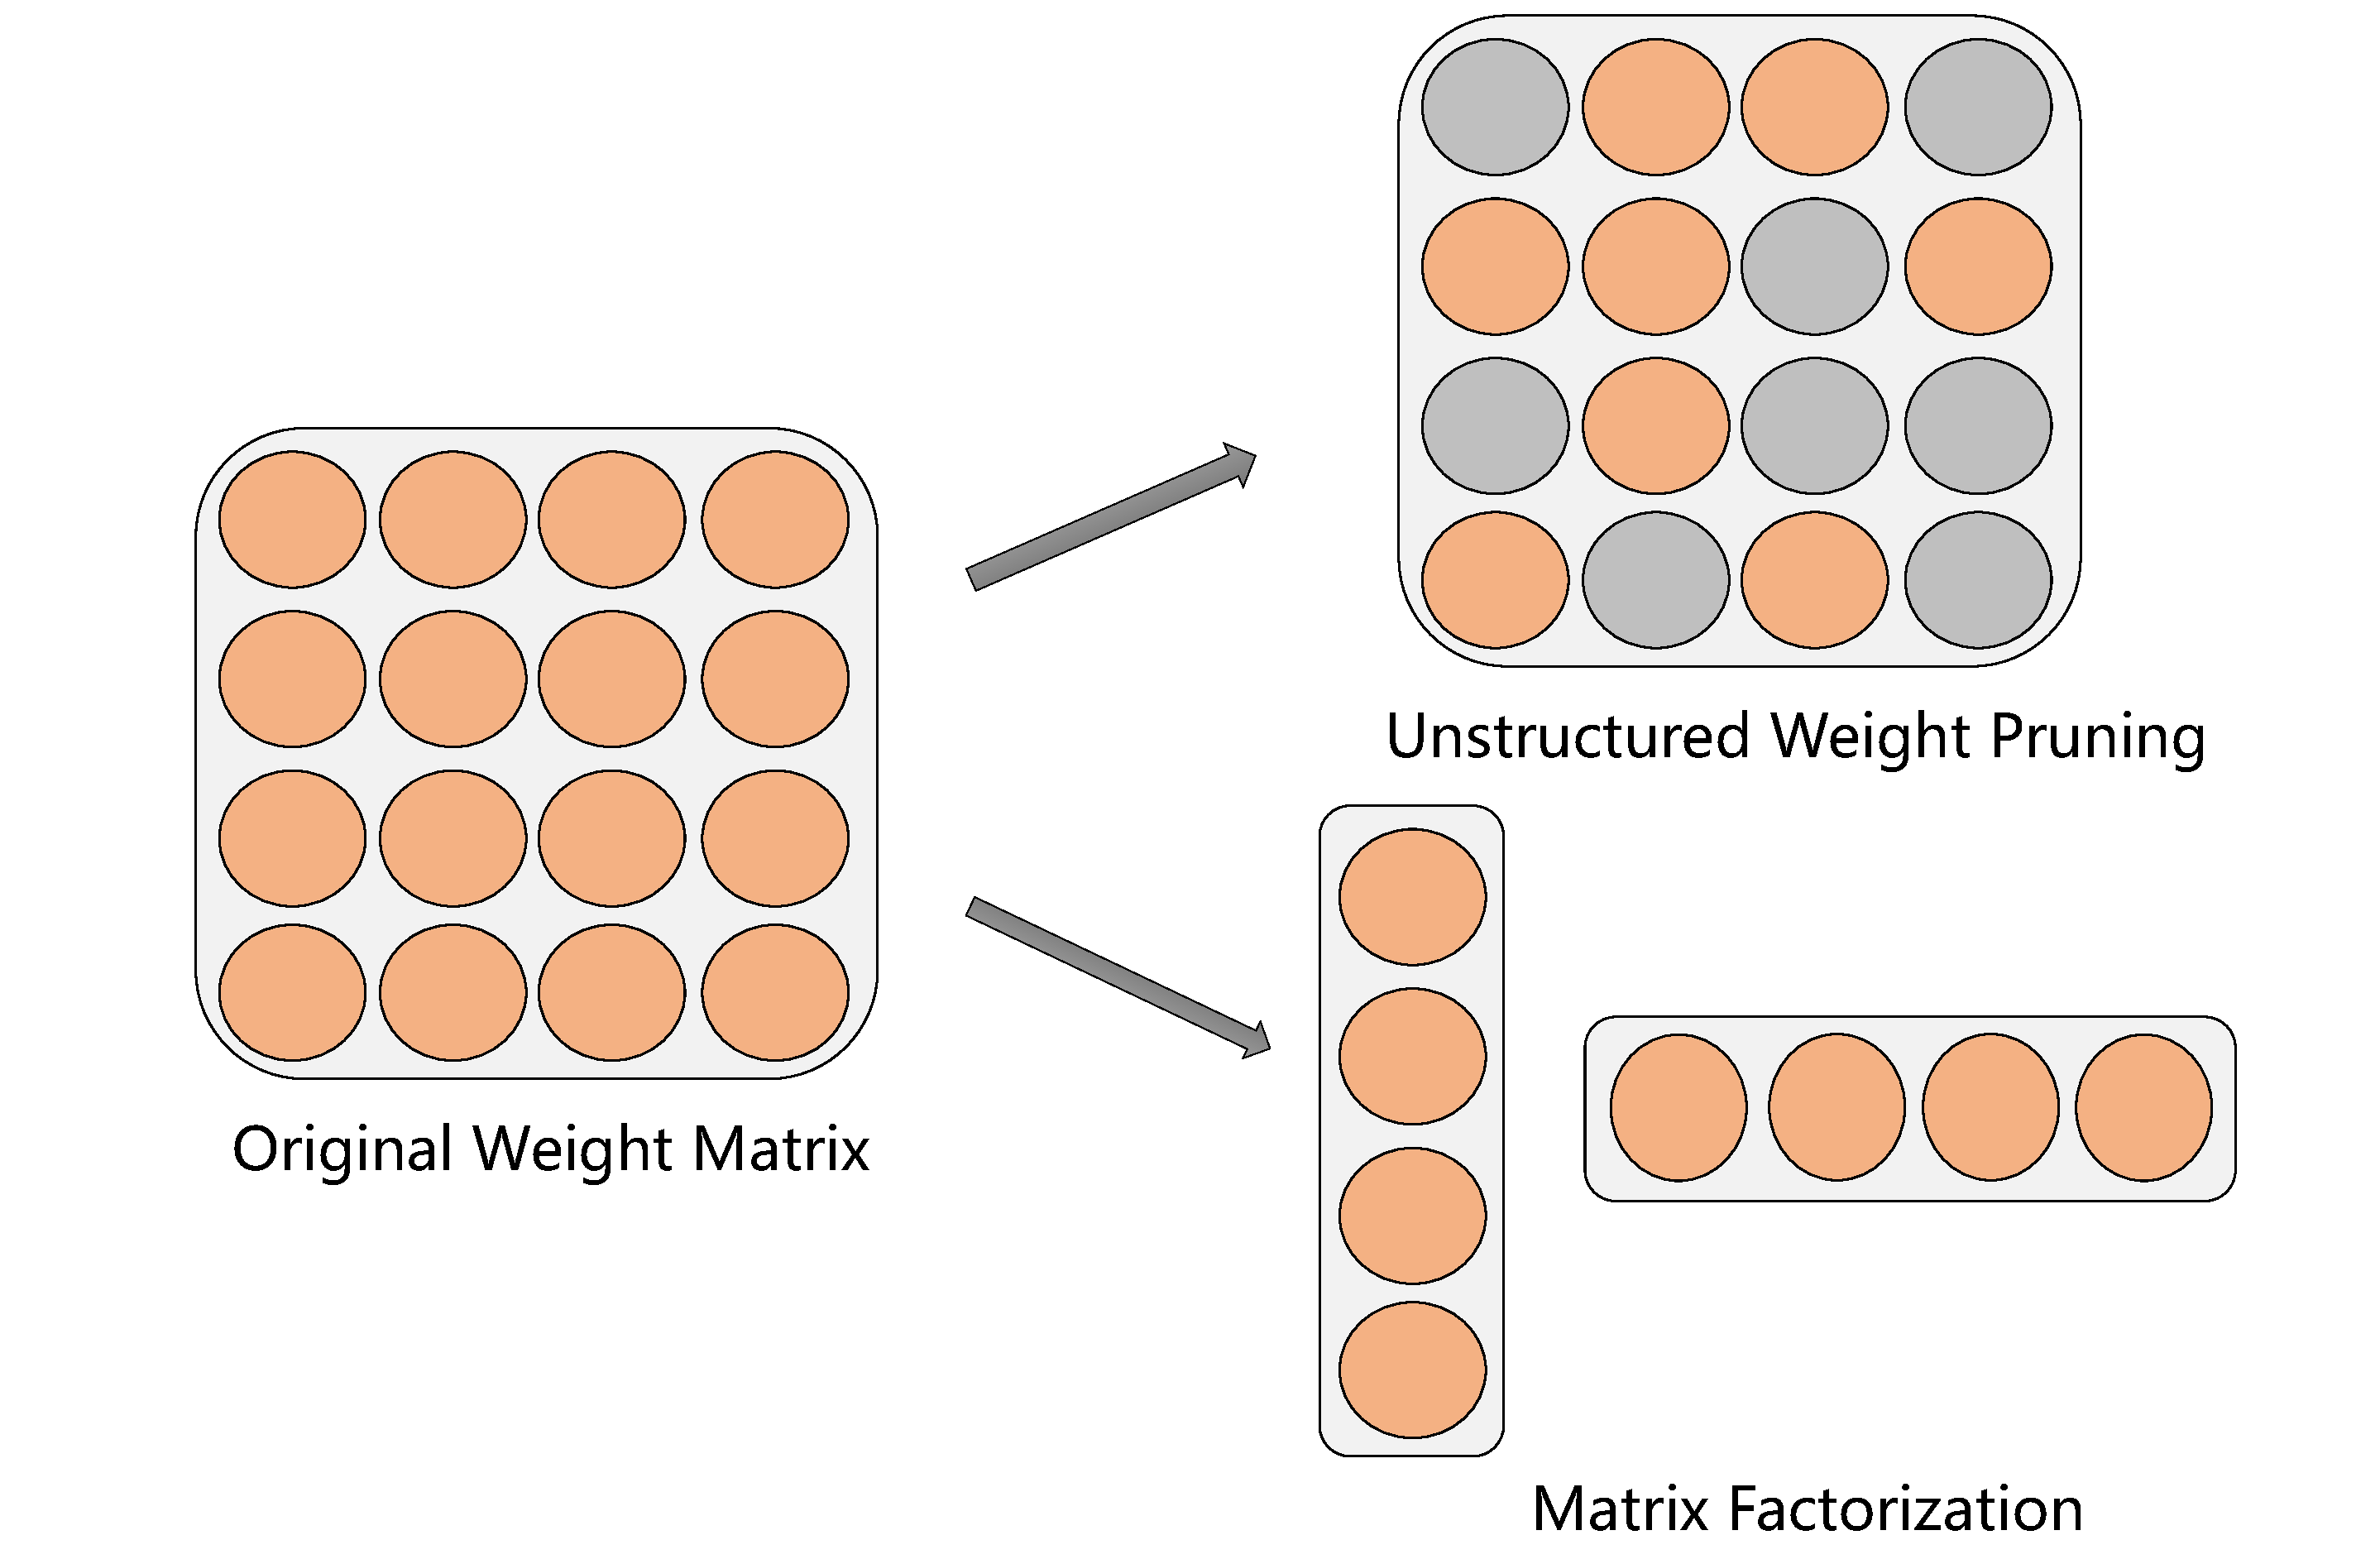
\includegraphics{./figures/intro_final.pdf}}
	\caption{Illustration of matrix factorization and unstructured pruning  on a single weight matrix.}
	\label{fig:intro}
\end{figure}

\subsection{Matrix Factorization~(MF)}
\label{sec:lr}
Given the weight matrix $\bm{W}\in \mathbb{R}^{n\times m}$, matrix factorization~\cite{svd} decomposes it into sub-matrices with reduced total number of parameters to achieve model compression.  
It first uses singular value decomposition~(SVD) to obtain an equivalent 
form of $\bm{W}$ as the product of three matrices:
\begin{align}
	\bm{W}=\bm{U}\bm{\Sigma}\bm{V}^\mathrm{T}
\end{align}
where $\bm{U}\in \mathbb{R}^{n\times r}$, $\bm{\Sigma}\in  \mathbb{R}^{r\times r}$, $\bm{V}\in \mathbb{R}^{r\times m}$, and $r$ is the rank of matrix $\bm{W}$. $\bm{\Sigma}$ is a diagonal matrix of non-zero singular values $\{\sigma_1, \sigma_2,...,\sigma_r\}$ in descending order. Then, low-rank approximation with targeted rank $k$ is obtained by keeping the top-$k$ singular values in $\bm{\Sigma}$ as well as their corresponding column vectors in $\bm{U}$ and $\bm{V}$:
\begin{align}
	\bm{W}&\approx \bm{U}_{[:, :k]}\bm{\Sigma}_{[:k,:k]}\bm{V}_{[:, :k]}^{\mathrm{T}} =\bm{A}\bm{B}
	\label{eq:svd}
\end{align}
where $\bm{A}=\bm{U}_{[:,:k]}\bm{\Sigma}_{[:k,:k]}$ and $\bm{B}=\bm{V}_{[:,:k]}^{\mathrm{T}}$ are the two final sub-matrices of which the product is used to replace $\bm{W}$. After such factorization, the number of parameters is reduced from $nm$ to $k(n+m)$. Different compression rates can be achieved by varying the preserved rank $k$.



\subsection{Unstructured  Pruning~(UP)}
\label{sec:pruning}
%We first establish some shared notations for unstructured weight pruning. 
Let $\bm{W}\in \mathbb{R}^{n\times m}$ denote a generic weight matrix in a PLM. In order to determine which elements in $\bm{W}$ are pruned, an importance score matrix $\bm{S}\in \mathbb{R}^{n\times m}$ is correspondingly introduced. The smaller $S_{i,j}$ is, the larger the probability of $W_{i,j}$ will be pruned. Given the importance scores, a pruning strategy $f_{prune}(\cdot)$ computes a binary mask matrix $\bm{M}\in \{0,1\}^{n\times m}=f_{prune}(\bm{S})$, 
and the forward process for an input $x$ becomes $y=(\bm{W}\odot\bm{M})x$, 
where $\odot$ denotes element-wise multiplication.

\paragraph{Zero-order Pruning~(UP$_{\text{zero}}$)} Zero-order pruning refers to the family of algorithms that only use the value of the weight as the importance measure.
For example, magnitude-based weights pruning~\cite{mag,chen2020lottery} adopts the absolute value of weight as importance score, i.e., 
$\bm{S}_{i, j}=|\bm{W}_{i, j}|$. The typical choice of $f_{prune}(\cdot)$ is to keep $v\%$  of weights with the largest importance scores:
\begin{align}
	\bm{M}_{i,j}=
	\begin{cases} 
		1, & \text{if }\bm{S}_{i,j}~\text{is in the largest }v\%\\
		0,  & \text{otherwise}  
	\end{cases}
	\label{eq:zero}
\end{align}


\paragraph{First-order Pruning~(UP$_\text{first}$)} Unlike zero-order pruning where $\bm{S}$ is directly derived from $\bm{W}$, first-order methods treat 
$\bm{S}$ as learnable parameters and jointly train it with model weights 
during fine-tuning. For example, SMvP~\cite{movement} and CAP~\cite{cap}
randomly initialize $\bm{S}$ and update it during the whole pruning process. The pruning strategy $f_{prune}(\cdot)$ is the same as in zero-order pruning~(\eqnref{eq:zero}).


%\begin{align}
%	\bm{M}_{i,j}=
%	\begin{cases} 
%		1, & \text{if }\bm{S}_{i,j}\ge \tau\\
%		0,  & \text{otherwise}  
%	\end{cases}
%	\label{eq:first}
%\end{align}
Since the gradient of the thresholding function is 0 everywhere, straight-through estimator~\cite{st} is used as an approximation. The importance score $\bm{S}_{i,j}$ of $\bm{W}_{i,j}$ up to training step $T$ can be expressed as: 
\begin{align}
\bm{S}_{i,j}=-\sum_{t\le T}(\frac{\partial \mathcal{L}}{\partial \bm{W}_{i,j}})^{(t)} \bm{W}_{i,j}^{(t)}
\end{align}
where $\mathcal{L}$ is the loss function. The formulation is also equivalent to the first-order Taylor approximation of the change in $\mathcal{L}$ if $\bm{W}_{i,j}$ is zeroed out.

\paragraph{Sparsity Scheduler}
The proportion of remaining weights is controlled by the sparsity scheduler, here  we adopt the commonly used  cubic sparsity schedule to progressively reach target sparsity, i.e., $v_t$ at time step $t$ is derived by:
\begin{align}
	%	v^{(t)}=
	\begin{cases} 
		v_i & t\in [0, t_i) \\
		v_f+(v_i-v_f)(\frac{T-t_{f}-t}{T-t_f-t_i})^3 & t\in[t_i, T-t_f) \\
		v_f  & \text{otherwise}  
	\end{cases}
\end{align}
\label{eq:prune}
where $v_i=1.0$, $v_f$ is the final percent of remained parameters, $t_i$ and $t_f$ are the warmup and cool-down steps. $T$ is the total training steps. Moreover, we discard $\bm{M}$ and directly set $\bm{W}_{i,j}$ to zero if $\bm{S}_{i,j}^{(t)}$ is not in the top-$v_t$ at time step $t$. 
%\paragraph{A Unified View} The differences in the implementation of 
%importance scores~(direct value inspection v.s. additional learnable 
%parameters) and pruning strategy~(top-$v$ selection v.s. tuned threshold) 
%make it hard to compare various pruning methods. To this end, 
%we establish a unified view of zero-order and first-order pruning, 
%denoted as \textbf{UWP$_\text{zero}$} and \textbf{UWP$_\text{first}$}, 
%with the only difference being the calculation of importance score $\bm{S}$.
%\KZ{This section is a little strange here because it seems to repeat
%what has been said in the previous subsections. You have already defined $S$
%but now you are singling out $S$ again. In particular, I can't appreciate why
%``it is hard to compare various pruning methods'', I don't really see
%the need for this unified view.}
%
%For UWP$_\text{zero}$, the calculation of $\bm{S}$ is the same as magnitude pruning, i.e., $\bm{S}_{i, j}^{(t)}=|\bm{W}_{i, j}^{(t)}|$, where $t$ is the time step. For UWP$_\text{first}$, we directly calculate its importance score $\bm{S}$ without introducing additional parameters, i.e.,  $\bm{S}_{i,j}^{(t)}=\bm{S}_{i,j}^{(t-1)}+|\frac{\partial \mathcal{L}}{\partial \bm{W}_{i,j}}^{(t)} \bm{W}_{i,j}^{(t)}|$. 

%\KZ{\eqref{eq:prune} seems 
%to be something new in this section but then it is part of the first-order 
%pruning, and nothing to do with zero-order pruning. So why is it in the 
%``unified view?''}

%\KZ{My feel is that this whole section of related work and background is a bit
%long-winded.}
 


\section{Preliminary Study}
\label{sec:pilot}
In this section, we conduct a preliminary study on unstructured pruning  and matrix factorization
based on BERT-base and try to find answers to the following two questions: (1) How does matrix factorization perform under high compression rates? (2) Do subnetworks produced by unstructured pruning contain \textit{low-rank} sparsity patterns while preserving the majority of task accuracy?
%\KZ{What kind of insight? You stop short of providing the motivation
%of the following experiments. Are you trying to see if these two methods alone
%work well to compress language model?}

\subsection{Experimental Setting}
\indent
\paragraph{Datasets}We use two tasks from GLUE benchmark~\cite{glue}, namely MRPC and RTE, as our evaluation testbeds. Both of them are formulated as classification problems.

\paragraph{Implementation Details} For matrix factorization, we follow the algorithm in \secref{sec:lr}. Specifically, we first fine-tune BERT-base on each downstream task following \citet{bert}. Then, we perform truncated SVD on weight matrices of each linear layer in the fine-tuned BERT and re-train the whole model to recover the lost accuracy. We select preserved rank $k$ from $\{390, 260, 130, 50\}$, which corresponds to $\{0.75, 0.50, 0.25, 0.10\}$ of BERT's parameters.

For unstructured  pruning, we evaluate both UP$_\text{zero}$ and UP$_\text{first}$. We set the value of $v_f$ from $\{0.75, 0.50, 0.25, 0.10\}$ to make a direct comparison to matrix factorization.

\subsection{Results and Analysis}
\label{sec:pilot_results}

%\begin{figure*}[t]
%	\centering
%	\scalebox{0.285}{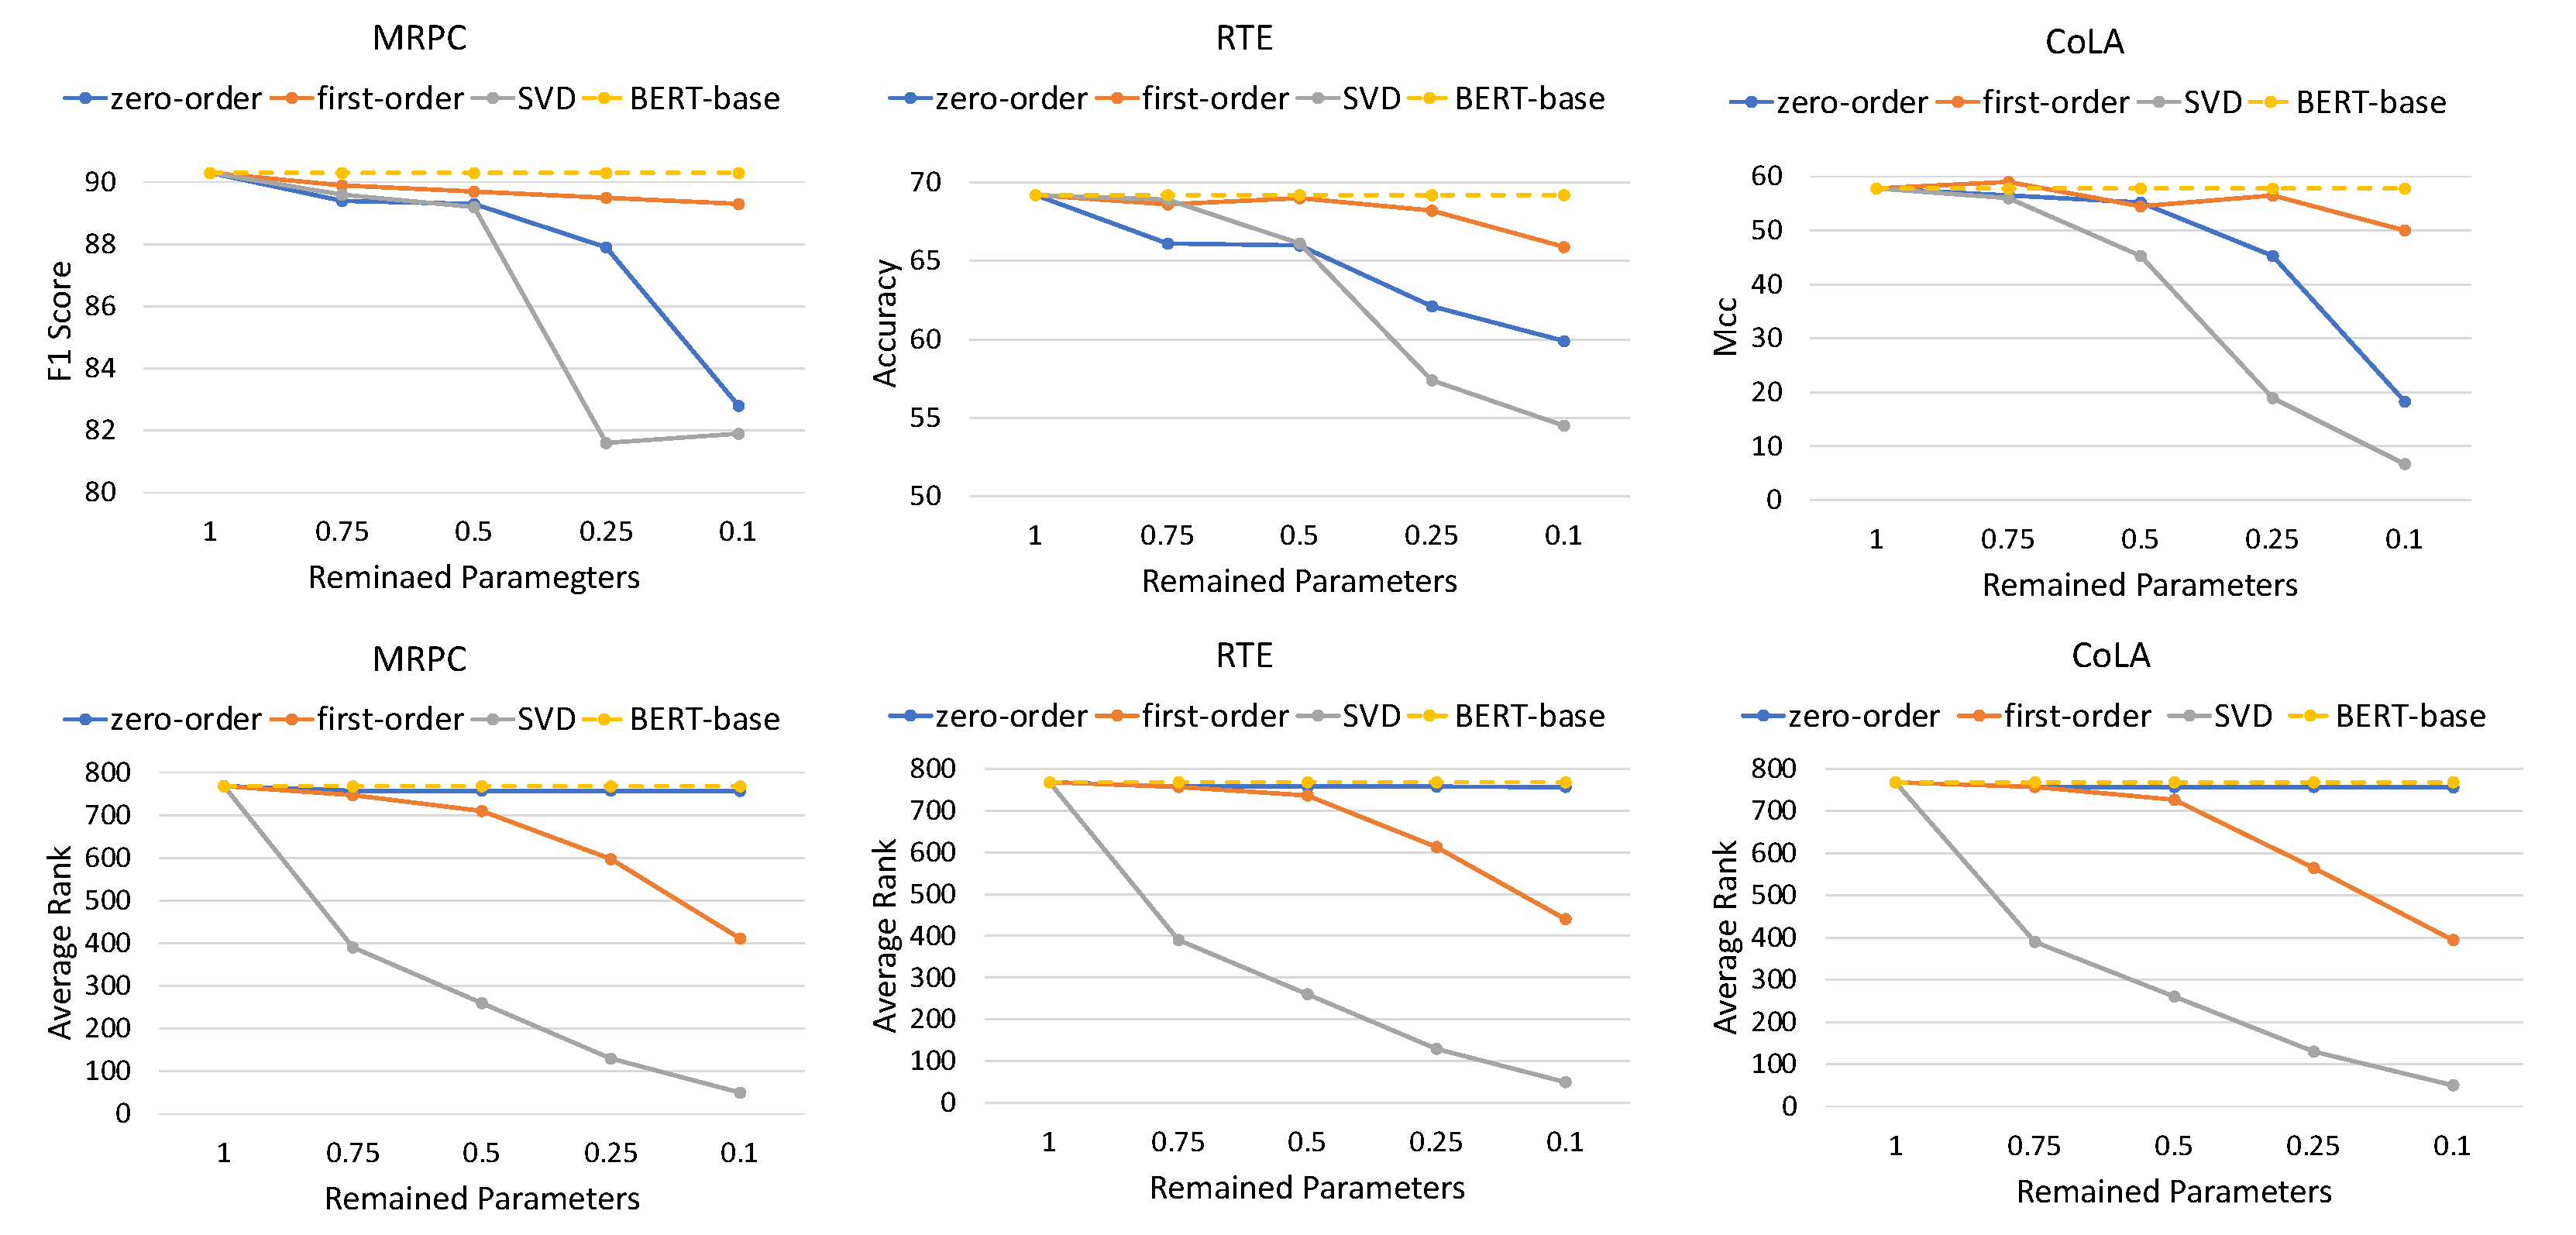
\includegraphics{./figures/pre_new.pdf}}
%	\caption{Task performance~(top half) and average matrix rank~(bottom half) v.s. percent of remained parameters. The dashed yellow line indicates the performance/rank upper bound by fine-tuning the full-scale BERT-base model.}
%	\label{fig:pre}
%\end{figure*}


\paragraph{Accuracy Preservation} 
The variation of task accuracy with respect to the remaining parameters is illustrated 
in the top half of \figref{fig:pre}. Under a small compression rate, i.e., 
$75\%$  parameters remaining, all examined methods can retain $\ge 97\%$ performance 
of BERT-base across all tasks. Under moderate compression rate, i.e., $50\%$ parameters remaining, UP$_\text{zero}$ and SVD start to show obvious declines. 
When more extreme compression rates are pursued, e.g., $25\%$-$10\%$ parameters 
remaining, SVD exhibits the most drastic performance drops compared to UP methods. 
On the contrary,  UP$_\text{first}$ still retains $\sim 97.6\%$ of BERT's performance.
UP$_\text{zero}$ lags behind UP$_\text{first}$ by a large margin under high sparsity. This indicates that magnitude alone cannot be used to quantify a weight's 
contribution because even a small weight can yield a huge influence on the model 
output due to the complicated compositional nature of neural networks. 
In contrast, the importance criterion of UP$_\text{first}$ directly reflects the 
sensitivity of the model's training loss w.r.t. each weight and is therefore more 
accurate.

\begin{figure}[t]
	\centering
	\scalebox{0.175}{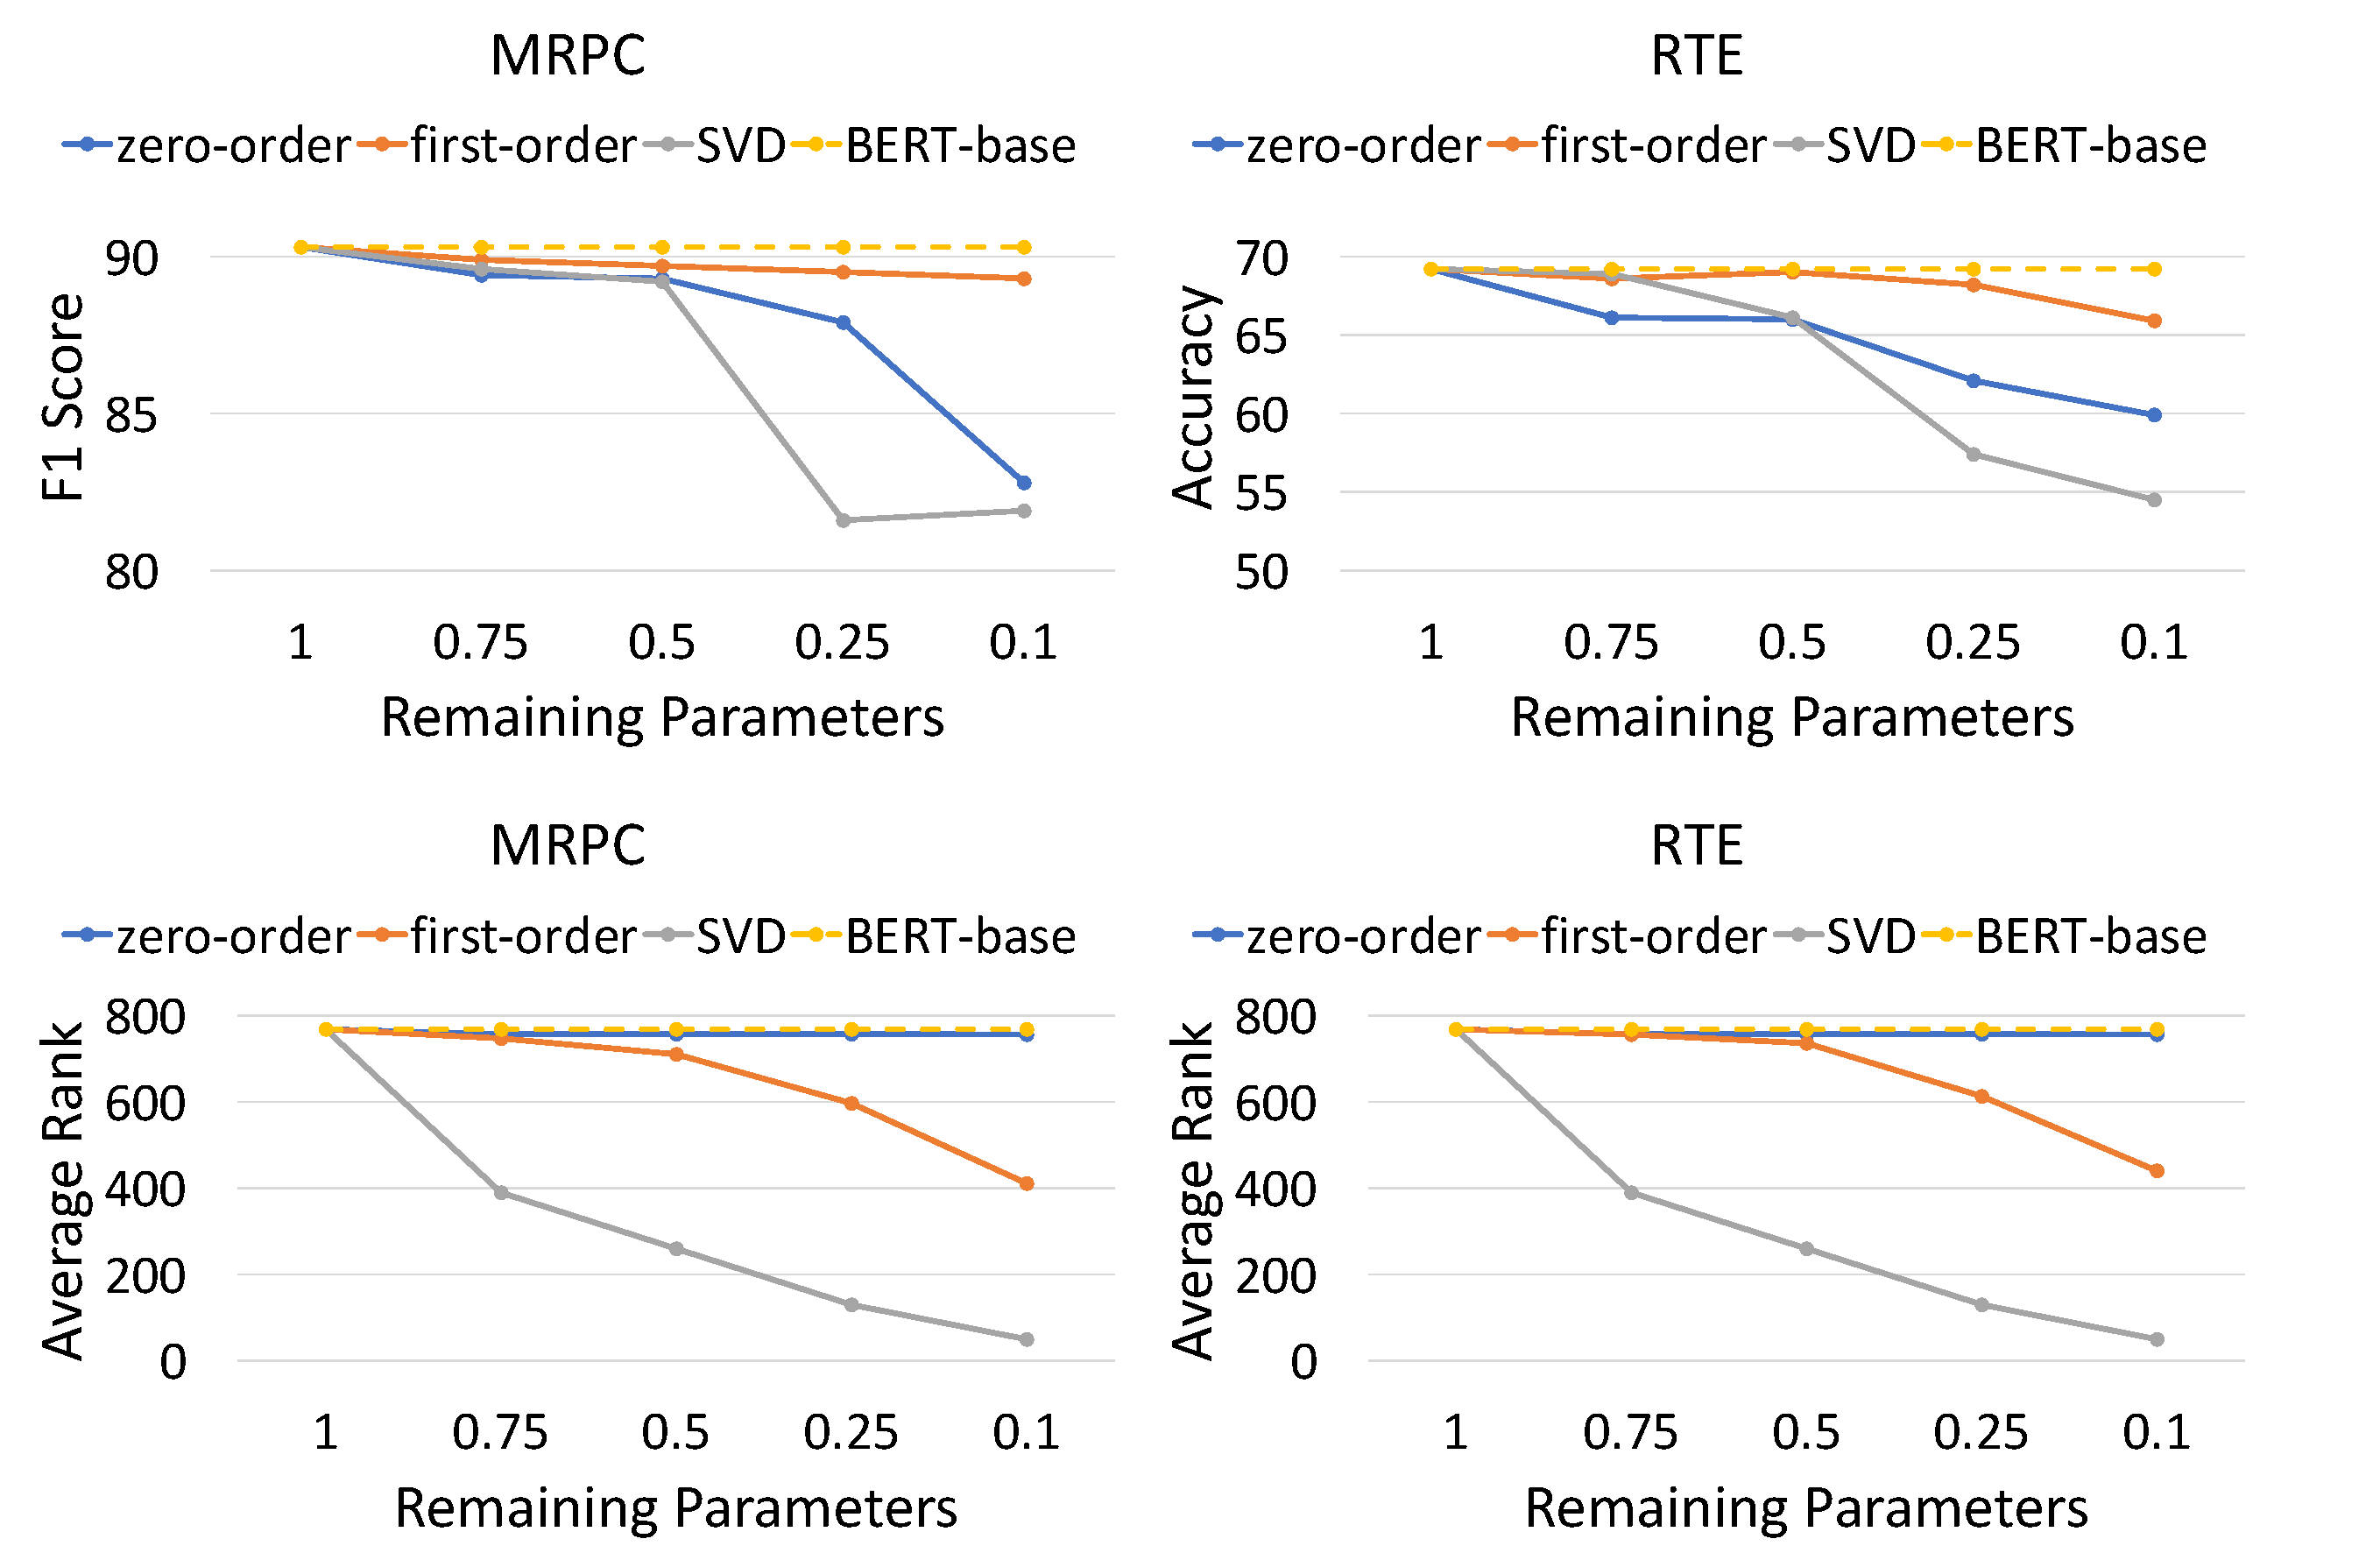
\includegraphics{./figures/pre_col.pdf}}
	\caption{Task accuracy~(top half) and average matrix rank~(bottom half) 
v.s. percentage of original parameters retained. 
The dashed line indicates the performance/rank upper bound by fine-tuning the full-scale BERT-base model. Results on more datasets are deferred to Appendix \ref{sec:A}.}
	\label{fig:pre}
\end{figure}

\begin{figure}[t]
	\centering
%	\scalebox{0.50}{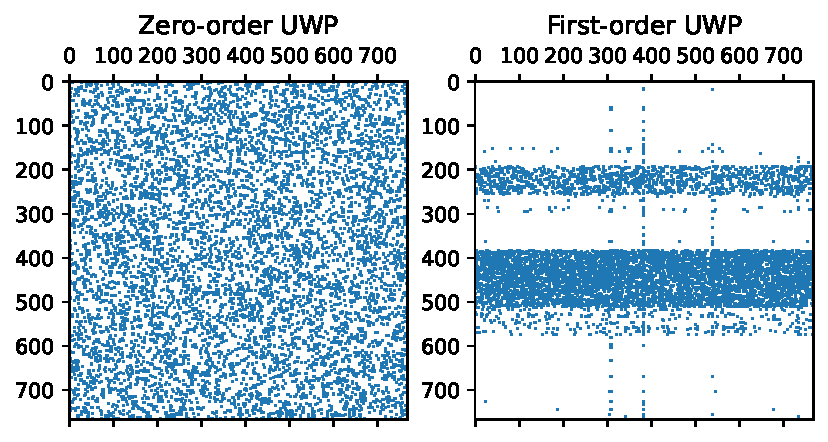
\includegraphics{./figures/sparsity_pattern.pdf}}
		\scalebox{0.50}{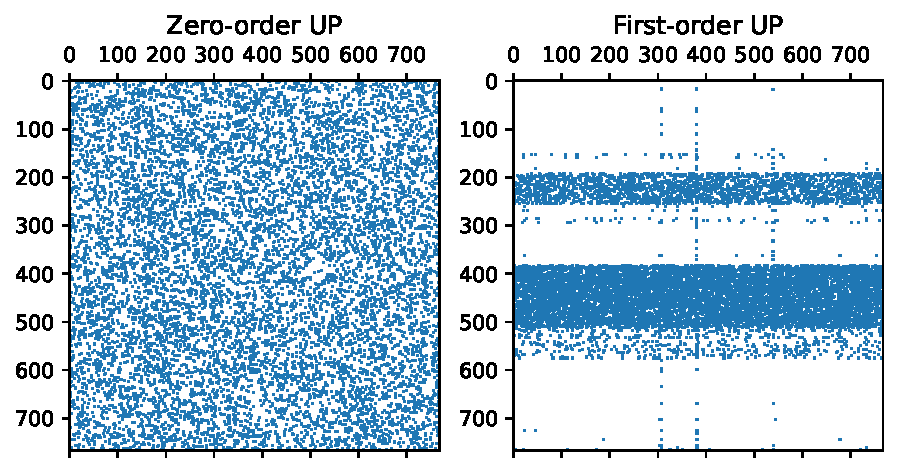
\includegraphics{./figures/zero_first_UP.pdf}}
	\caption{Sparsity patterns of the same 768x768 weight matrix  pruned by UP$_\text{zero}$~(left) and UP$_\text{first}$~(right) on MRPC with $10\%$ of
the parameters remaining.}
	\label{fig:pattern}
\end{figure}

\paragraph{Rank} 
Considering the inferior accuracy of SVD, we hypothesize that the weight matrices of fine-tuned BERT are high-rank, 
hence leading to a large approximation error when $k$ is small. The bottom half of \figref{fig:pre} inspects the average rank of weight matrices. We can see that the weight matrices in fine-tuned BERT-base are nearly full-rank, which explains the inefficacy of SVD when $k$ is small. We also plot the rank-parameter curve of UP methods. For UP$_\text{zero}$, it produces sparse matrices that are 
as high-rank as densely fine-tuned BERT even when $90\%$ weights are set to zero. In contrast, UP$_\text{first}$  produces sparse patterns whose rank monotonically decreases as more weights are pruned. To gain more insights into this phenomenon, we visualize the weight matrix pruned by UP$_\text{zero}$ and UP$_\text{first}$ in \figref{fig:pattern}. Though both are designed without structural bias,  unlike UP$_\text{zero}$, UP$_\text{first}$ learns to remove entire rows from the weight matrix and 
the resulting matrix enjoys a low-rank characteristic.



\begin{figure}[th]
	\centering
	\scalebox{0.142}{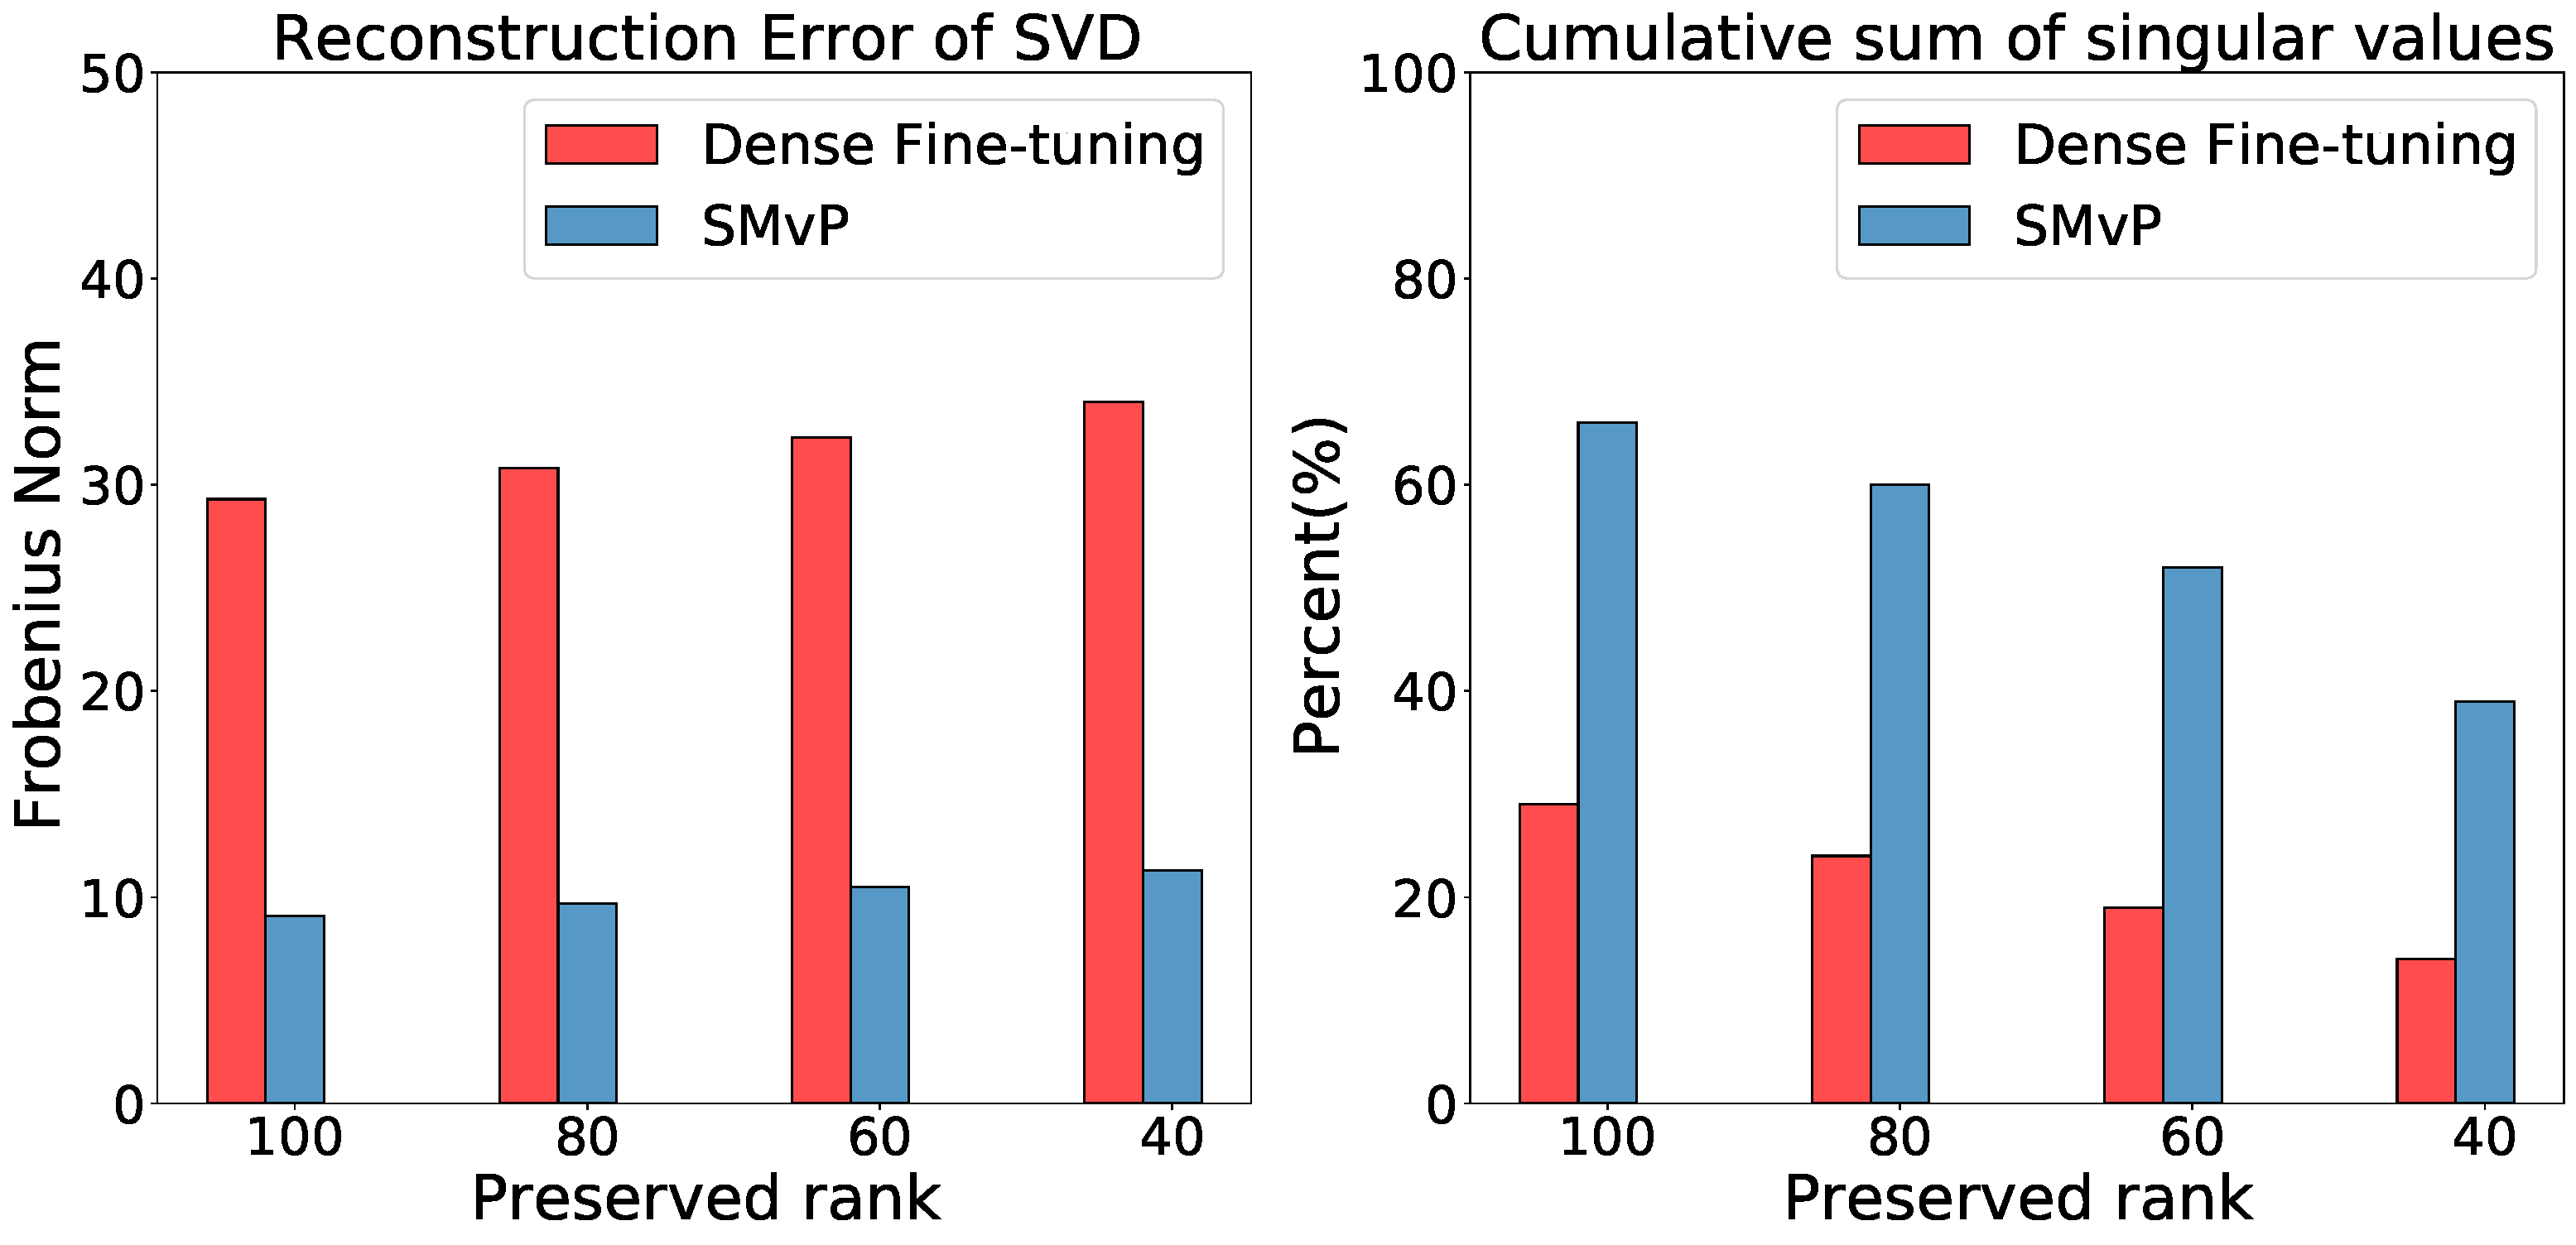
\includegraphics{./figures/norm_vis.pdf}}
	\caption{Quantitatively measuring approximation quality via reconstruction error~(left) and cumulative sum of singular values~(right) on MRPC.}
	\label{fig:norm}
\end{figure}

\paragraph{The Idea}
%\KZ{The key insight is: factorize a high-rank matrix into low rank sub-matrices
%loses a lot of info, but factorize a low-rank matrix into low rank sub-matrices
%doesn't lose as much info. Our design is based on this insight. I think as long
%as you make this insight clear, that's good enough. Some of this section
%is a bit verbose.} 
%Given the fact that factorizing from a low-rank matrix into sub-matrices loses less information than factorizing from a high-rank matrix
%Given the competitive task performance and low-rank structure of UWP$_\text{first}$, 
%it appears plausible to perform low-rank matrix factorization on 
%low-rank sparse models for model compression. 
The key insight is: factorizing a high-rank matrix into low rank sub-matrices
loses significant quantity of useful information, but factorizing a low-rank matrix into low rank sub-matrices
doesn't lose as much information. Our design is based on this insight. 
As a sanity check of its feasibility, we quantitatively measure the 
quality of low-rank approximation with various preserved ranks $k$. 
\figref{fig:norm} shows that given a specific $k$, 
the sum of top-$k$ singular values of matrices produced by UP$_\text{first}$ takes a much larger portion of total values than fine-tuning, suggesting that we can reserve more information of low-rank sparse matrix given the same $k$. The reconstruction error~(measured by Frobenius norm) of UP$_\text{first}$ is also significantly lower, implying a higher approximation quality. We thus expect that low-rank matrix factorization on low-rank sparse models to effectively combine: 
(1) the good performance of first-order UP; 
(2) direct memory and computation reduction by MF.

\section{LPAF: Low-rank Prune-And-Factorize}
\label{sec:approach}
Here we formally propose the LPAF~(\textbf{L}ow-rank \textbf{P}rune-\textbf{A}nd-\textbf{F}actorize) framework 
for language model compression. In addition, 
we propose two optimizations in the 
initialization and training of the compression process.

\subsection{The Overall Workflow}
\label{sec:ptf}
Given a pre-trained language model $T$ and a downstream task with training set $D=\{(x_i, y_i), i=1,2,...M\}$, LPAF consists of three steps to realize model compression: 
\begin{itemize}
	\item Step-1: obtaining the low-rank sparse model $T_{\text{sparse}}=\text{UP}_\text{first}(T,D, v)$. $v$ is the percent of remained parameters after pruning.
	\item Step-2:  performing matrix factorization on each weight matrix~(excluding the embedding layer) in $T_{\text{sparse}}$ and  obtain its low-rank factorized form $T_{\text{factorized}}$. 
	%	The perceivable reduction of model's memory footprint and computation cost happens at this step.
	\item Step-3:  re-training $T_{\text{factorized}}$ on $D$ using task-specific loss function until convergence. 
	%	Since step 2 inevitably loses certain task-specific information, this step is designed to ensure that the compressed model retain good task performance.
\end{itemize}

Next, we present two novel optimizations, namely \textit{sparsity-aware SVD} and \textit{mixed-rank fine-tuning}, that improves the matrix factorization and fine-tuning process in step 2 and step 3 respectively.

\subsection{Optimization 1: Sparsity-aware SVD}
\label{sec:sasvd}
SVD has been shown~\cite{bestsvd} to provide the optimal rank-$k$ approximation to $\bm{W}$ with respect to the Frobenius norm:
\begin{align}
	\nonumber
	\min_{\bm{A},\bm{B}} ||\bm{W}-&\bm{A}\bm{B}||_{F}=\min_{\bm{A},\bm{B}} \sum_{i,j}(\bm{W}_{i,j}-(\bm{AB})_{i,j})^2 \\
	& \text{s.t.}~~~~\text{rank}(\bm{AB})=k
\end{align}
It is a generic factorization method in that it is applicable to any matrix $\bm{W}$ by penalizing the reconstruction error of each individual weight equally. 

In our case, $\bm{W}$ is a sparse matrix from $T_{\text{sparse}}$ in which the majority of weights are set to zero by the pruning algorithm $P$. These zero weights are deemed to have less impact on the task performance compared to the retained~(unpruned) weights. However, the vanilla SVD treats each weight equally without considering the inherent sparseness of $W$, thus may be sub-optimal for preserving useful information in $W$ about the end task.
To address this issue, we propose sparsity-aware SVD which considers different priorities of parameters and weighs the individual reconstruction error based on its importance score $\bm{S}_{i,j}$:
\begin{align}
	\min_{\bm{A},\bm{B}} \sum_{i,j}&\bm{S}_{i,j}(\bm{W}_{i,j}-(\bm{AB})_{i,j})^2~~~\\\
	 & \text{s.t.}~~\text{rank}(\bm{AB})=k
	\label{eq:sasvd}
\end{align}
In this way, parameters that are more important can be better reconstructed, hence retaining more task performance from $T_{\text{sparse}}$ at initialization. Nevertheless, \eqnref{eq:sasvd} does not have a closed form solution~\cite{weightedsvd,hsu2021language} when each $\bm{W}_{i,j}$ has its own weight. We therefore resort to a simplification by letting the same row of $\bm{W}$ share the same importance. The importance for row $i$ is given by $\hat{\bm{S}}_{i}=\frac{\sum_{j}\bm{S}_{i,j}}{\sum_{n}\hat{\bm{S}}_{n}}$. Let $\hat{\bm{I}}=diag(\hat{\bm{S}}_1,\hat{\bm{S}}_2,...,\hat{\bm{S}}_{n})$ denote a diagonal matrix,  \eqnref{eq:sasvd} is now converted to:
\begin{align}
	&\min_{\bm{A},\bm{B}}||\hat{\bm{I}}\bm{W}-\hat{\bm{I}}\bm{A}\bm{B}||_F~~~~
	\\
	& \text{s.t.}~~\text{rank}(\bm{AB})=k
\end{align}
This essentially amounts to applying rank-$k$ SVD upon $\hat{\bm{I}}\bm{W}$, i.e., $\hat{\bm{I}}\bm{W}=\hat{\bm{U}}\hat{\bm{\Sigma}}\hat{\bm{V}}^\mathrm{T}$. Then the solution of $\bm{A}$ and $\bm{B}$ can be analytically obtained by:
\begin{align}
	\bm{A} &= \hat{\bm{I}}^{-1}\hat{\bm{U}}_{[:,:k]}\hat{\bm{\Sigma}}_{[:k,:k]},\bm{B}=\hat{\bm{V}}_{[:,:k]}^{\mathrm{T}}
\end{align}


\subsection{Optimization 2: Mixed-rank Fine-tuning}
Recall that the last step of LPAF is to fine-tune $T_{\text{factorized}}$ on the training set $D$. This process has been proven essential to regain the performance lost during factorization~\cite{svd}. However, during the experiments, we observe the performance of fine-tuned $T_{\text{factorized}}$ still slightly lags behind $T_{\text{sparse}}$ given a similar parameter budget. 
%\KZ{Isn't it normal for $T_{factorize}$ to lag behind $T_{sparse}$? Is there any evidence (experimental results) to show
%this ``lagging''?  Even in Fig. 3, in most cases, $T_{sparse}$ is still better Ours. 
%So I don't see enough motivation for this Mixed-rank fine-tuning.} 
We posit that, due to the reduced capacity~(less trainable parameters) and model-level approximation error incurred by low-rank factorization, joint fine-tuning of low-rank matrices may converge to sub-optimal solutions with lower generalization ability. To mitigate this problem, we propose mixed-rank fine-tuning, a regularized scheme for training low-rank matrices.

Let $\{(\bm{A}\bm{B})_i, i=1,2...,N\}$ denotes all low-rank matrices in $T_{\text{factorized}}$. During training, for each $(\bm{A}\bm{B})_i$, we sample a binary Bernoulli random variable $z_i\sim \text{Bernoulli}(p)$, where $p$ is a global hyper-parameter. Then, the local computation process involving $(\bm{A}\bm{B})_i$ is modified to:
\begin{align}
	\bm{x}_{out} = (1-z_i)*(\bm{A}\bm{B})_i \bm{x}_{in} + z_i * \bm{W}_i\bm{x}_{in} 
\end{align}
where $\bm{W}_i$ is the sparse matrix in $T_{\text{sparse}}$ from which $\bm{A}_i$ and $\bm{B}_i$ are derived. In this way, the low-rank matrices can further 
benefit from gradient-level regularization from  $T_{\text{sparse}}$, 
thus reducing the generalization gap. The hyper-parameter $p$ is controlled by a scheduler. We implement it such that $p$ is linearly decayed from an initial value $p_{\text{init}}$ to zero by a constant step size $d$:
\begin{align}
	p = \text{max}(0, p_{\text{init}}-d*t)
\end{align}
As $p$ decreases, $\bm{W}_i$ is gradually substituted by low-rank sub-matrices $(\bm{AB})_i$. When $p$ reaches zero, the training enters the phase of standard fine-tuning. To further mitigate the training instability brought by sampling, we let each input go through the forward pass twice with different $\bm{z}^1=\{z_i^1\}_{i=1}^{N}$ and $\bm{z}^2=\{z_i^2\}_{i=1}^{N}$, and impose a consistency objective on the two outputs to promote stability:

\begin{align}
	\mathcal{L}_{c}=\mathcal{D}(y_{\bm{z}^1}, y_{\bm{z}^2})
\end{align}
where $\mathcal{D}$ can be the KL divergence for classification tasks and the MSE loss for regression tasks.

% After $p$ reaches zero, the model still benefits from the regularization effect brought by different dropout masks~\cite{rdrop}.

\section{Prompt Design}
\label{sec:method}
% We describe the iterative methodology of designing prompts with users' feedback, which will be listed in bullet point in this section. 

% Our prompt engineering for chatbots was based on (i) the objectives proposed by psychiatrists (see Section \ref{sec:objectives}), (ii) the process of ``trial and error'', and (iii) the feedback of psychiatrists. In this part, we will discuss the design process in detail.
% \KZ{I'm assuming in the trial and error stage, you will involve
% the human doctors and patients and get their feedback. But how is this process
% actually playing out? How is it different from the final evaluation which also
% consists of human and automatic evaluation. It's a little confusing.
% I think sec 4 - 7 need to be re-organized according to the two-stage
% methodology and redesign what to put into the final evaluation section.}
% In this part, we will discuss the design process in detail.
Based on the objectives obtained in Phase 1, we started prompt engineering, which is always iterative and full of ``trial and error''.

\subsection{Design Methodology}
When designing prompts for a chatbot, it is common practice to involve humans in conversing with the chatbot for each version of the prompt. However, common applications can involve general public as human judges, while in our practice, real users (i.e., doctors and patients) are necessary to be involved to meet the requirements of real-world applications. While human engagement is essential for prompt engineering, it can also make the iterative design process time-consuming and resource-intensive.

Inspired by \citet{deriu-etal-2020-spot}, we utilize a ``bot-to-bot'' method to generate dialogue history and collect user feedback based on it. 
% \KZ{One potential issue with bot-to-bot approach, is that the initial
% version of the doc bot and patient bot must be good enough to generate
% reasonable logs.} 
Instead of the conventional ``bot-to-human'' approach, we facilitate autonomous conversations between the doctor chatbot and the patient chatbot. By leveraging this autonomous interaction, we generate dialogue history that reflects potential user interactions. These generated chat logs are then presented to real psychiatrists, who provide valuable feedback and insights based on their expertise. 
This approach allows us to simulate user interactions without requiring direct human involvement, thereby reducing the time and resources needed for the iterative design process. Moreover, we can make informed improvements and refine the chatbot in subsequent iterations by incorporating the input of healthcare professionals.

\subsection{Doctor Chatbot}
\label{sec:doc_prompt}
As illustrated in  \figref{fig:doc_prompt_design}, we undergo three iterations to develop the prompt for the doctor chatbot, and the final version is presented below:
\begin{prompt}
    \ding{192} Please play the \uline{role} of an \uline{empathetic and kind} psychiatrist. 
    \ding{193} Your \uline{task} is to conduct a professional diagnosis conversation with me based on the DSM-5 criteria. 
    \ding{194} Your questions should \uline{cover at least the following aspects}: [\ldots]\protect\footnotemark. 
    % You are free to choose the order of questions, but you must collect complete information on all aspects in the end. 
    \ding{195} Please only ask \uline{one question at a time}.
    % , and each question should only cover one symptom.
    \ding{196} You need to ask \uline{in-depth questions}, such as the \Blue{duration}, \Blue{causes} and specific \Blue{manifestations}. 
    \ding{197} You need to use various \uline{empathetic strategies}, such as \Yellow{understanding}, \Yellow{support} and \Yellow{encouragement}. 
\end{prompt}
\footnotetext{The aspects include ``emotion'', ``sleep'', etc. We provide the full list in Appendix \ref{apd:prompts}.}

\begin{figure}[th]
	\centering
	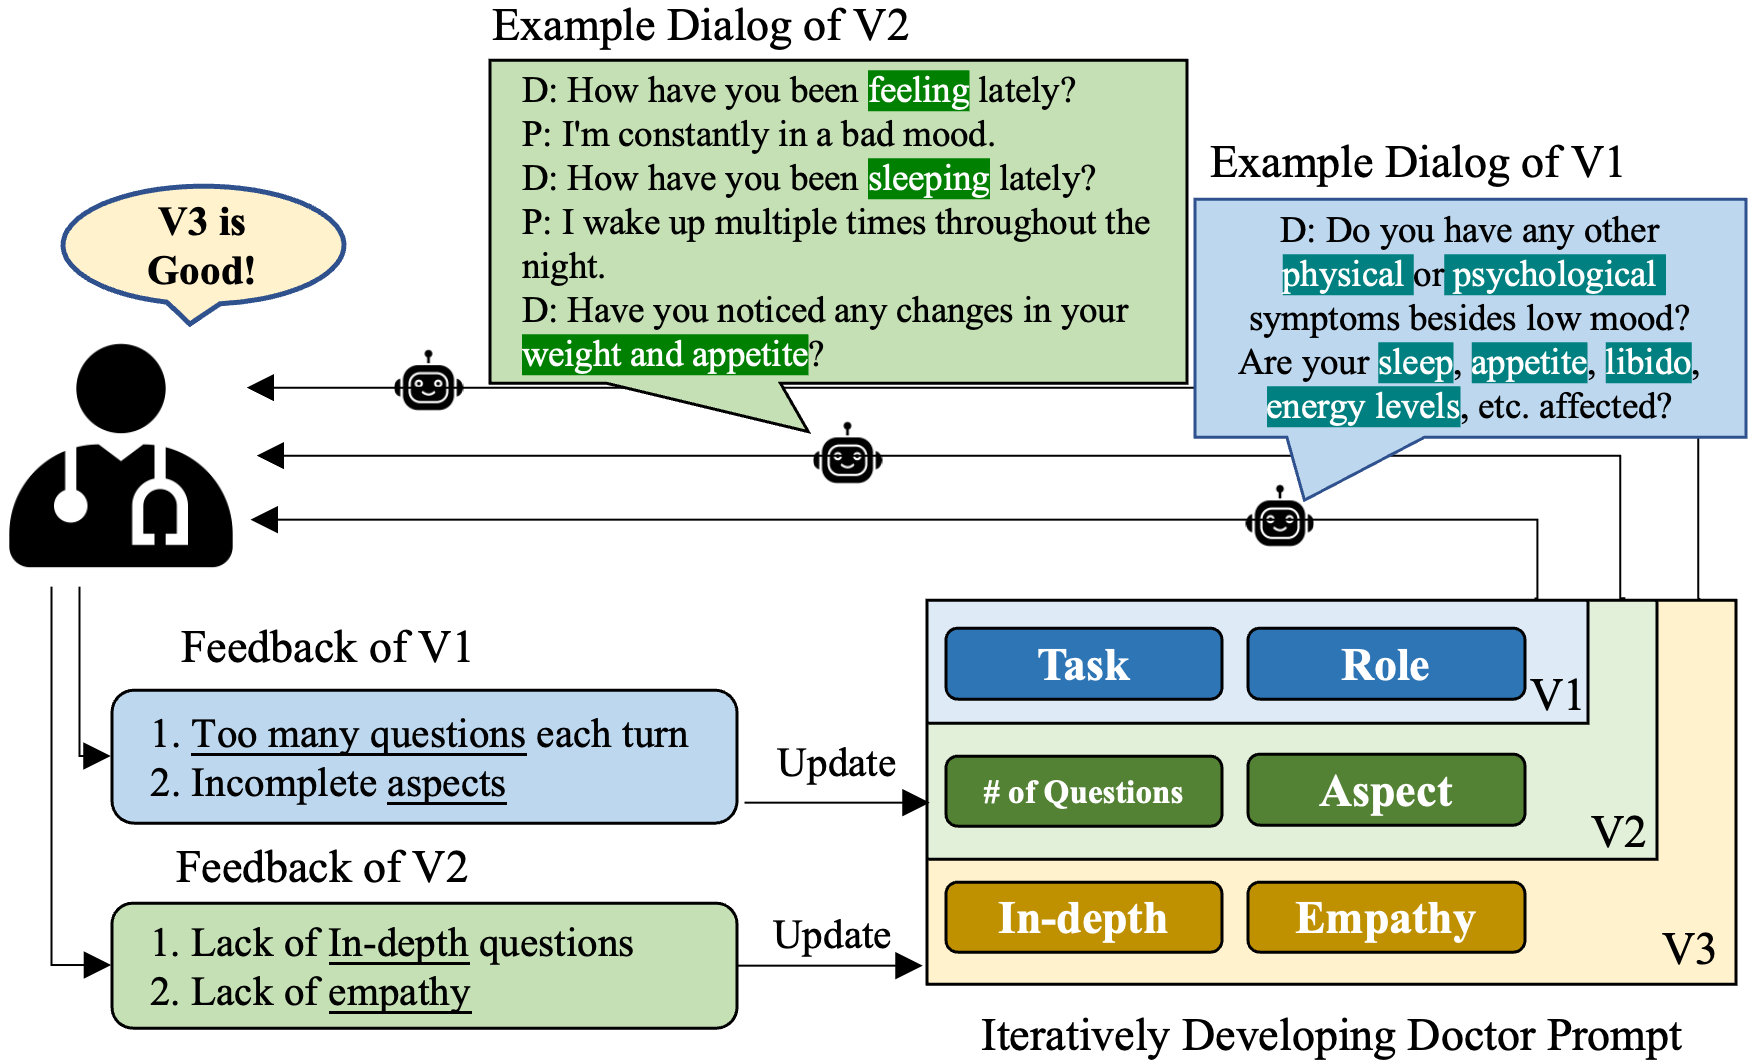
\includegraphics[width=\linewidth]{Figures/doctor_prompt_design.png}
	\caption{The iterative development process of the prompt of doctor chatbots. Psychiatrists will identify the limitations of the current version, and we will address these issues in the subsequent version.}
	\label{fig:doc_prompt_design}
\end{figure}
In this prompt, we provide a clear description of the task and establish the role to be simulated by the doctor chatbot. Then, we list the specific aspects that the doctor chatbot should cover during the questioning process. This serves as a guideline to ensure the \textit{comprehensiveness} objective. What's more, we include examples (highlighted in colored boxes) in the prompt to guide the doctor chatbot in asking \textit{in-depth} questions and demonstrating \textit{empathy}. These examples are crucial because, without them, the chatbot tends to ask superficial questions and  rely on generic phrases like ``thank you very much for your answer'' to show empathy. This arises from ChatGPT's limited comprehension of ``in-depth questioning'' and ``empathy'' in clinical contexts. Consequently, providing examples can be a promising approach to help ChatGPT grasp certain specialized skills within professional domains.

\subsection{Patient Chatbot}
\label{sec:pat_prompt}
After two iterations, we arrive at the final version of the prompt for the patient chatbot, which is presented below:
\begin{prompt}
    \ding{192} Please play the \uline{role} of a patient, who is currently chatting with a doctor. 
    \ding{193} \uline{You are experiencing the following symptoms}: [\texttt{Symptom List}]\protect\footnotemark 
     % \KZ{Instead of giving the full list of symptoms in the prompt, shouldn't we give a random subset of those symptoms?}
    \ding{194} Please talk to me based on the above symptom list. 
    \ding{195} You can only mention \uline{one symptom per round}. 
    \ding{196} You should \Blue{express} your symptoms in a \uline{vague and colloquial} way, and relate them to your \uline{life experiences}.
    \ding{197} You can have \Blue{emotional fluctuations} during the conversation. 
    \ding{198} You have a \Blue{resistance} towards doctors, and do not want to reveal some feelings easily.
\end{prompt}
\footnotetext{The symptom list is summarized by ChatGPT and revised by psychiatrists. See Appendix \ref{apd:symp_list} for details.}

In the first iteration, we describe the task (sentence \ding{192}\ding{193}), provide a symptom list (sentence \ding{194}) in the prompt, and add sentence \ding{195} to avoid listing all the symptoms in one turn. 
This prompt enables the chatbot to meet the basic requirement of providing \textit{honest} responses in most cases.
However, feedback from psychiatrists indicates that the chatbot lacks resemblance to real patients as it does not effectively convey \textit{emotions}, use colloquial \textit{expressions}, or demonstrate \textit{resistance} to seeking help. 

Therefore, we add sentence \ding{196}, \ding{197}, \ding{198} to address these issues in the second iteration.
However, we observe that the effect of adding these sentences is most prominent in the initial rounds of conversation, suggesting that the patient chatbot tends to forget some of the instructions given at the beginning. 
This behavior is reasonable considering ChatGPT's training objective to be a helpful, polite AI assistant that provides detailed responses. Consequently, there can be a potential mismatch between the desired behavior of the patient chatbot, including resistance and emotional fluctuations, and the training objective, making it more likely for these instructions to be forgotten.

To address this issue, we insert new reminders during the conversation. Inspired by the fact that the latter part of the prompt has the greatest impact on the responses generated by ChatGPT, our method is straightforward yet effective. Without users' awareness, we covertly append the following words at the end of the most recent sentence in the dialogue history.

\begin{prompt}
    (\Yellow{Attention:} colloquial language, life experience, low mood or mood swings, refuse or answer briefly due to resistance)
\end{prompt}

We aim to use simple phrases or words as reminders during the conversation to ensure that the sentences are not overly long. Moreover, these reminders are only temporarily attached to the most recent round, and will not persist in the dialogue history for subsequent rounds.
% With these reminders, the patient chatbot can maintain a colloquial language style consistently and exhibit resistance even in the latter part of the conversation, so we consider this version as the final one\footnote{The final version is in Table \ref{tab:patient_prompt} in Appendix \ref{apd:prompts}.}.


\section{Evaluation Framework}
\label{sec:eval_frameworks}
% \KZ{Are we only evaluating the final version of the two bots from prev section? This is not part of the iterative design process right? This should be made clearer.}
% \MY{normally we provide objective/automatic eva first, followed by human evaluation results. when introducing the metrics and results, follow this order}

Guided by psychiatrists and through an iterative development process, we established the objectives for two chatbots and completed their designs in Phase 2. In addition, we also designed an evaluation framework, which will be employed in Phase 3 to assess the performance of the developed chatbots. This section will describe our evaluation framework which encompasses interactive experiments for human evaluation and various task-specific metrics.
\subsection{Chatbots of Comparison}
% \KZ{this section should go into the evaluation framework?}

Due to the complexity and high time cost of human evaluation, we select several representative prompt versions for comparison, and discuss the evaluation process of doctor and patient chatbots respectively.

\paragraph{Doctor Chatbot} 
Each patient will have a conversation with four different doctor chatbots in a random order, and then rate them on four human evaluation metrics with 1-4 scale. 
Three of the chatbots are powered by ChatGPT. \texttt{D1} uses the full prompt, 
while the other two (i.e., \texttt{D2}, 
\texttt{D3}) have certain parts removed for ablation. 
The fourth chatbot, \texttt{CPT}, is a representative deep learning chatbot trained on domain-specific data \cite{yao-etal-2022-d4} using CPT model~\cite{shao2021cpt}. 
% \MY{Make a table for these bots, including doctor and patient}
\paragraph{Patient Chatbot}
Each psychiatrist will have a conversation with two patient chatbots, and then rate their performance with 1-4 scale. 
The two patient chatbots are \texttt{P1} and \texttt{P2}, aligning with the prompt versions in Section \ref{sec:pat_prompt}. 
A brief description of these chatbots can be found in Table \ref{tab:cmp_chatbots}.
% The first one uses the full prompt while the second one omits additional parts for realistic in version 2\footnote{Detailed description and prompt of these doctor/patient chatbots are shown in Appendix \ref{apd:prompts}.}.
% COMMENT: 这两段要引述一下表1啊。此外1中的"xx parts"的表述,最好和前面一致,都用v1v2v3或者①②③这种方式来提,更容易理解。CPT这个模型的名字也应该在正文里写出来。

\begin{table}[h]
    \centering
    \footnotesize
    \begin{tabular}{m{0.1\columnwidth}|c|m{0.6\columnwidth}}
    \hline
    & Chatbot & Description \\
    \hline
    \multirow{4}{0.1\columnwidth}{Doctor} & D1 & use the full doctor prompt \\
    \cline{2-3}
    & D2 & remove empathy parts in prompt  \\
    \cline{2-3}
    & D3 &  remove aspect part in prompt \\
    \cline{2-3}
    & CPT & CPT model trained on domain data \\
    \hline
    \multirow{2}{0.1\columnwidth}{Patient} & P1 & use the prompt in the first iteration \\
    \cline{2-3}
    & P2 & use the full patient prompt\\
    \hline
    \end{tabular}
    \caption{Brief description of the chatbots for comparison. Detailed description and prompt is in Appendix \ref{apd:prompts}.}
    \label{tab:cmp_chatbots}
\end{table}
\subsection{Evaluation Metrics}
\label{sec:eval_metric}
When designing evaluation metrics, our goal is to ensure that each objective is accompanied by appropriate metrics for accurate measurement.  We employ both human and automatic metrics for evaluation, and divide the automatic metrics of both kind of chatbots into two types: \textbf{function} and \textbf{style}. The overview of these metrics and their relations to objectives can be found in \figref{fig:all_metric}.
% \MY{Clearer now, but still mixing function and style - which objectives and metrics are function-related and which are style?}.
% NEWCOMMENT: 这里这样分类之后,在图中也要把两类指标区分出来,可以在objective那一列上做区分
\begin{figure}[th]
	\centering
	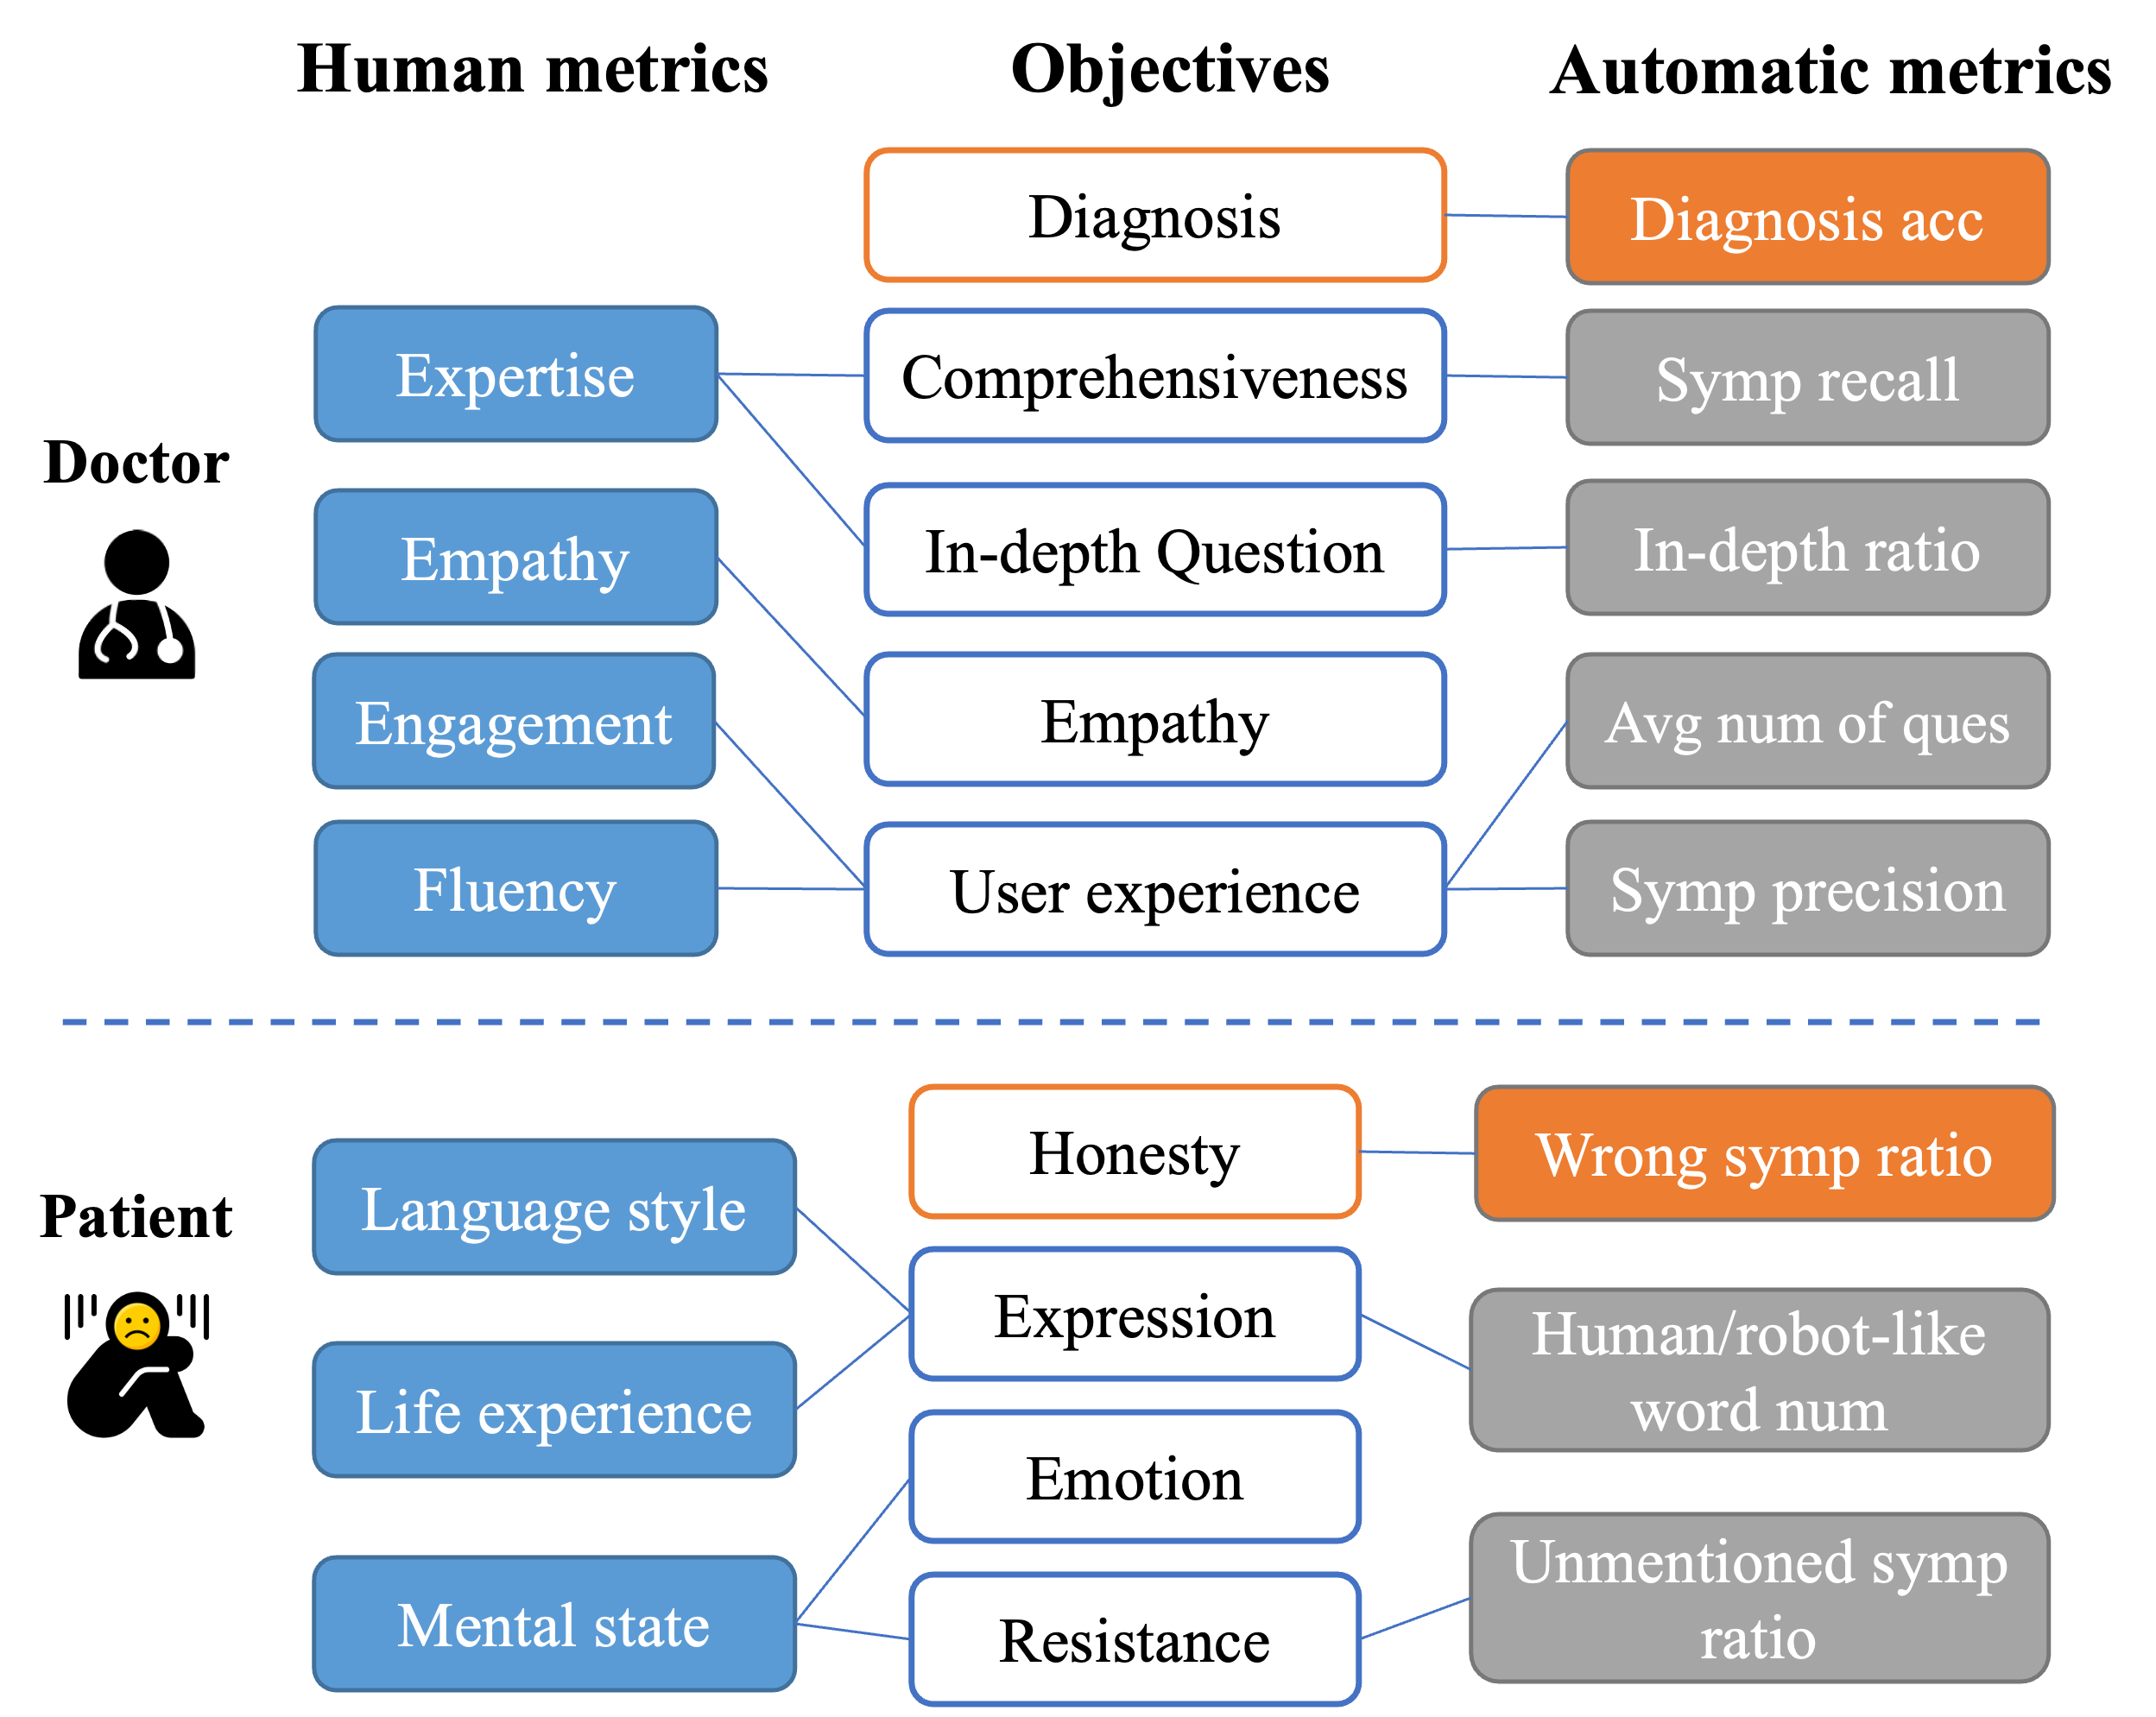
\includegraphics[width=\linewidth]{Figures/metrics.png}
	\caption{The correspondence between evaluation metrics and objectives. \textbf{\textit{Function}} metrics are orange, and \textbf{\textit{style}} metrics are gray.}
	\label{fig:all_metric}
\end{figure}

\subsubsection{Metrics for Doctor Chatbot}
\label{sec:doc_metric}
\paragraph{Human evaluation} In most cases, patients do not have specialized knowledge in psychiatry, making it difficult for them to assess a doctor's professional skills precisely. Therefore, when designing human evaluation metrics for doctor chatbots, we focus mainly on the user experience. The metrics are shown in Table \ref{tab:human_eval_doctor}.
\begin{table}[h]
    \centering
    \footnotesize
    \begin{tabular}{m{0.18\columnwidth}|m{0.7\columnwidth}}
    \hline
    Metrics & Explanation \\
    \hline
    Fluency & The chatbot does not repeat previously asked questions and can smoothly switch between different topics. \\
    \hline
    Empathy & The chatbot can understand and comfort you properly. \\
    \hline
    Expertise & The chatbot behaves like a real doctor, making you believe in its professionalism. \\
    \hline
    Engagement & The chatbot can maintain your attention and make you want to continue talking to it. \\
    \hline
    \end{tabular}
    \caption{Human evaluation metrics of doctor chatbot.}
    \label{tab:human_eval_doctor}
\end{table}
\paragraph{Automatic evaluation}
Different from human evaluation metrics, we mainly measure the expertise of the doctor chatbot using automatic metrics. 
The \textit{functional} requirements for doctor chatbot is to provide an accurate diagnosis, so the corresponding metric is \uline{``diagnosis accuracy''}. 
The \textit{style} part concerns the doctor chatbot's professional skills. We use \uline{``symptom recall''} to evaluate the chatbot's ability to comprehensively gather the patient's symptom-related information, and use \uline{``in-depth ratio''} to assess the ability to ask in-depth questions for deeper understanding. 
To ensure a better user experience, we calculate the \uline{``average number of questions''} asked in a single interaction to discourage the chatbot from overwhelming patients with excessive queries. Furthermore, we employ the metric of \uline{``symptom precision''} to penalize the chatbot's mechanistic behavior of asking all potential questions, irrespective of the user's responses. 

\subsubsection{Metrics for Patient Chatbot}
\label{sec:pat_metric}
\paragraph{Human evaluation}
There is no standard to measure whether a patient is ``good'' enough. Thus, when chatting with patient chatbots, doctors can only assess whether their style of expression and manner of communication resemble real patients enough and whether they can describe their symptoms in a reasonable way, so the main metrics for human evaluation are \textbf{Resemblance} and \textbf{Rationality}.
What's more, we divide the Resemblance metric into three aspects in Table \ref{tab:human_eval_patient}, according to the objectives in Section \ref{sec:objectives}.

\begin{table}[h]
    \centering
    \footnotesize
    \begin{tabular}{m{0.18\columnwidth}|m{0.65\columnwidth}}
    \hline
    Metrics & Explanation \\
    \hline
    Mental State & The chatbot is in depressed state, such as be in low mood, reluctance to communicate, scattered thoughts, etc.\\
    \hline
    Life Experience & The description of symptoms is related to daily life and personal experiences.\\
    \hline
    Language Style & Use colloquial and natural expressions when describing symptoms.\\
    \hline
    \end{tabular}
    \caption{Three aspects of the ``Resemblance'' metric.}
    \label{tab:human_eval_patient}
\end{table}
\paragraph{Automatic evaluation}
The \textit{functional} requirement of patient chatbot is ``honesty'', and we can calculate \uline{``wrong symptom ratio''} by comparing the patient's symptom list with the symptoms it reported to assess this aspect. 

Then, we evaluate the patient chatbots' \textit{style} using some linguistic features, like \uline{``Human/robot-like word ratio''}, to find out whether their language is colloquial with limited usage of professional terminology. We also use \uline{``unmentioned symptom ratio''} to measure the resistance level of chatbots. 

\subsubsection{Computation and Annotation}
A detailed explanation of the automatic metrics for the doctor and patient chatbot can be found in Appendix \ref{apd:eval}. 
In addition, to calculate some of these metrics, we need to annotate the dialogue history. This involves identifying the relevant symptom in the doctor's question, determining whether the patient truly experiencing a certain symptom, and so on, which is described in Appendix \ref{apd:annotation}.
Due to the inadequacy of dialogue history data for training multiple classification models, we employ ChatGPT to automatically label each sentence in the dialogue history, leveraging its impressive annotation capabilities~\cite{Gilardi2023ChatGPTOC}. Subsequently, three annotators thoroughly review and rectify the results to ensure the quality of the annotation.
% To assess the performance of dialogue systems, it is crucial to employ both human evaluation and automatic metrics, especially in mental health domain. Since there is little previous work on how to evaluate simulated psychiatrists and patients, we design several task-specific metrics and interactive experiments for human evaluation. 

\subsection{Human Evaluation Participants}
% We first implemented a website to host our chatbots, making it easier for participants to interact with them and rate their performance. The details of the website can be found in Appendix \ref{sec:chatInterface}. 
%\subsubsection{Participants}
In contrast to the approach of using actors/actresses to simulate patients as mentioned in \citet{yao-etal-2022-d4}, our evaluation process involves actual depression patients and psychiatrists, enabling us to assess the performance of chatbots in real-world scenarios.

Depression patients are recruited through online advertisements.
A total of 14 volunteers completed the entire process, with ages ranging from 18 to 31, and male and female participants accounted for 28.57\% and 71.43\% respectively. 
To assess the severity of their depression, patients are asked to complete the Beck Depression Inventory~\cite{beck1996beck}. Notably, we have a balanced distribution of healthy, mild, moderate and severe depression subjects which distribution is presented in Table \ref{tab:distribution_seve} in Appendix \ref{apd:eval}.
% \KZ{If the severity is ``none'', this patient is considered healthy?}

We invited 9 psychiatrists who are not involved in the prompt design, through cooperation with hospitals. Two of them are graduate students majoring in psychiatry, and the rest are practicing psychiatrists with rich clinical experience to ensure the professionalism of the evaluation.
% \footnote{Detailed information about these psychiatrists is in Appendix.}. 
% \KZ{Better provide anonimized version of their affiliations in the appendix, to make these people more credible?} \MY{Agree with Kenny's comment here, we can include their affiliation and how many years of expertise in this field}




% To ensure the quality of the dialogue data and evaluation, we also utilize a series of quality control strategies, which can be found in Appendix \ref{apd:quality}.


% COMMENT: 自动评测是如何实现的,如何自动把“症状”和“诊断结果”从对话中抽取出来,应该需要在这里说明一下



\section{Data Collection}
\label{sec:data}

To the best of our knowledge, available large scale 3D Bin Packing order dataset is very rare, especially with real-sized items. For that purpose, we create a dataset on 3D bin packing problem of real-world E-commerce platform. This L3DBPD consists of two parts: the customer order data is collected from Taobao\footnote{\url{https://www.taobao.com/}} E-commerce platform and item size data (with length, width and height) is collected from Cainiao\footnote{\url{https://www.cainiao.com/}} Logistics platform. We randomly sampled 150,000 training data and 150,000 testing data for customer orders with 8, 10 and 12 items, which are named as BIN8, BIN10 and BIN12 respectively. We use one line to demonstrate one customer order.

\begin{table*}[!h]
	\small
	\centering
	\caption{Examples of L3DBPD. }
	\label{dataset table}
	\begin{tabular}{|c| c | c | c | c | c | c | c | c | c |}
		\hline
		Order ID & item1  & item2 & item3 & item4  & item5 & item6 & item7  & item8  &  baseline \\  \hline
		1   & (140,50,180) & (100,70,60)  & (170,150,40) & (130,70,40) & (190,150,20)  & (190,150,20) & (240,200,160) &
		(160,170,50)  & 432600  \\ \hline
	\end{tabular}
\end{table*}


Take Table \ref{dataset table} as an example of BIN8, the first and last columns indicate the order ID of a customer order and the heuristic baseline of this BPP, the contents of the remaining 8 columns respectively shows the length, width and height of each items that belong to this order.
We believe this dataset will contribute to the future research of 3D bin packing problem. \footnote{The data will be published soon after accepted.}

\section{Experiment Evaluation}
\label{sec:experiment}
In this section, we first give some statistics of our corpus and evaluate the quality and quantity of the learned rules. Then, we compare with other causal knowledge bases. Next, we analyze and discuss some main sub-modules in the rule learning framework. Finally, a practical application of futures price prediction and demonstration are introduced. Our experiments are implemented in Python and SWI-Prolog\footnote{ \url{ http://www.swi-prolog.org/}}.
% and run on a computer with Intel Xeon 32 CPU(2.60GHz) and 173GB memory.
	
\subsection{Dataset}
We crawled the text dataset from Chinese financial news website \footnote{\url{ http://finance.sina.com.cn}}. The news data containing 4,991,000 articles, from 2000/7/20 to 2017/12/31, is used to rule learning.
%	, which are split into \textbf{111,330,205} sentences. The number of unique sentences is \textbf{75,572,053}, covering  \textbf{67.88\%} of the total sentences. 
The number of sentences with causal cue words is 7,147,141, accounting for 9.46\% of the total number of de-duplicated sentences (75,572,053. The repetition rate of sentences is about 32\%).
It shows that about  \textbf{14.2\%} (9.64\%/(1-32\%)) sentences explicitly express causality in online financial news sentences.
The news data containing 270,562 articles, from 2018/1/1 to 2018/11/2, is used to evaluate our framework. We set $\alpha$ to 0.5 to achieve an equal balance between generalization and specialization in rule induction. 
We set $\gamma$ to 0.3 to control the Prolog engine to reason around two steps, since more than two steps lead to obviously unreasonable results.

%	\begin{table}[]
%		\caption{Dataset Information}
%		\begin{center}
%		\begin{tabular}{|l|l|l|}
%			\hline
%			Dataset       & Train & Test \\ \hline
%			Time Interval &       &      \\ \hline
%			Number        &       &      \\ \hline
%		\end{tabular}
%	\end{center}
%	\end{table}

\subsection{Rule Evaluation}
We evaluate these rules both quantitatively and qualitatively.
\paragraph{Quantitative Evaluation}
The number of the final rules we learned is \textbf{50000}. We divide the rule quality into three levels: good, fair and bad. According to the ranking of rule confidence, we randomly select 200 rules from the top 10000 rules and manually divide them into three levels. The `good', `fair', and `bad' levels of them account for \textbf{32.5\%}, \textbf{39.0\%} and \textbf{28.5\%}, respectively.
%	\begin{table}[]
%		\centering
%		\begin{tabular}{|l|l|l|} \hline
%		 good & fair &bad \\ \hline
%			65/200(32.5\%)& 78/200(39.0\%) & 57/200(28.5\%) \\ \hline
%		\end{tabular}
%		\caption{Rule Quality}
%		\label{tab:rule_quality}
%	\end{table}

\paragraph{Qualitative Evaluation}
%\begin{align*}
%%	good
%%	{"c": ["过剩_1", "X_燃料", "产量", "", ""], "e": ["下降_1", "X_自然资源", "价格", "", ""], "relation": [["c_sc", "e_sc", "madeof"]], "ctx": {"senids": [1975666], "pattern_ids": [8]}, "ruleid": 5131, "confidence": 0.5657637042081998}
%&\text{1 (X, '产量/yield', '过剩/surplus', '', ''):-(Y, '价格/price', '下降/fall',} \nonumber\\
%&\text{'',''), IsA(X, '燃料/fuel'), IsA(Y, '自然资源/natural resource'),} \nonumber\\
%&\text{madeof(X, Y)} \\
%%{"c": ["结束_1", "X_国家", "罢工", "", ""], "e": ["下降_1", "X_金属", "价格", "", ""], "relation": [["e_sc", "c_sc", "atlocation"]], "ctx": {"senids": [341012], "pattern_ids": [6]}, "ruleid": 11607, "confidence": 0.5824045924950126}
%&\text{2 (X, '罢工/strike', '结束/stop', '', ''):-(Y, '价格/price', '下降/fall', }\nonumber\\
%&\text{'',''), IsA(X, '国家/nation'), IsA(Y, '金属/metal')}\nonumber\\
%&\text{, atlocation(Y, X)}	 \\
%%{"c": ["下降_1", "X_作物", "价格", "", ""], "e": ["减少_1", "", "", "X_作物", "面积"], "relation": [["c_sc", "e_oc", "=="]], "ctx": {"senids": [961411], "pattern_ids": [8]}, "ruleid": 978, "confidence": 0.5876590112986869}
%&\text{3 (X, '价格/price', '下降/fall', '', ''):-(X, '面积/area', '减少/fall', }\nonumber\\
%&\text{'',''), IsA(X, '作物/crop')} \\
%%fair
%%2{"c": ["下降_1", "X_国家", "储蓄率", "", ""], "e": ["下降_1", "X_国家", "增长率", "", ""], "relation": [["c_sc", "e_sc", "=="]], "ctx": {"senids": [1640122], "pattern_ids": [5]}, "ruleid": 213, "confidence": 0.7185889172176277}
%&\text{4 (X, '储蓄率/saving rate', '下降/fall', '', ''):-(X, '增长率/growth rate', }\nonumber\\
%&\text{'下降/fall','',''), IsA(X, '国家/nation')} \\
%%2{"c": ["下降_1", "", "X_产品", "", ""], "e": ["适合_1", "", "X_作物", "", ""], "relation": [["c_s", "e_s", "madeof"]], "ctx": {"senids": [1791763], "pattern_ids": [6]}, "ruleid": 19783, "confidence": 0.5634539402859007}
%&\text{5 ('', X, '下降/fall', '', ''):-('', Y, '适合/fit', '', ''), IsA(X, }\nonumber\\
%&\text{'产品/product'), IsA(Y, '作物/crop'), madeof(X, Y)}   \\
%%bad
%%1{"c": ["减少_1", "", "X_国家", "X_自然资源", "依赖性"], "e": ["增加_1", "", "", "X_燃料", "销量"], "relation": [["e_oc", "c_oc", "madeof"]], "ctx": {"senids": [1707156], "pattern_ids": [8]}, "ruleid": 4468, "confidence": 0.5717182258485046}
%%另一方面,由于日本、韩国和中国减少对中东地区进口原油的依赖性,道达尔公司希望增加对这三个国家的液化天然气销量。
%&\text{6 ('', X, '减少/fall', Y, '依赖性/dependence'):-('', '', '增加/increase',}\nonumber\\
%&\text{ Z,'销量/sales'), IsA(X, '国家/nation'), IsA(Y, '自然资源/natural-} \nonumber\\
%&\text{resource'), IsA(Z, '燃料/fuel'), madeof(Z,Y)}	
%\end{align*}
Figure \ref{fig:rules_case} shows some typical rules: 1,2,3 are good, 4,5 are fair, and 6 is bad.
The main problems of these rules include:
The extracted events are not incomplete, which makes the rules less informative, such as rule 4 and 5.
The causality between cause event and effect event is not very strong, which should be attributed to the design of causal patterns and the process of rule induction, such as 4 and 6.
Some other problems also exist, such as verb disambiguation when normalizing predicates, noun disambiguation when generalizing rule instances.
%	\begin{figure}[htbp]
%	\begin{center}
%		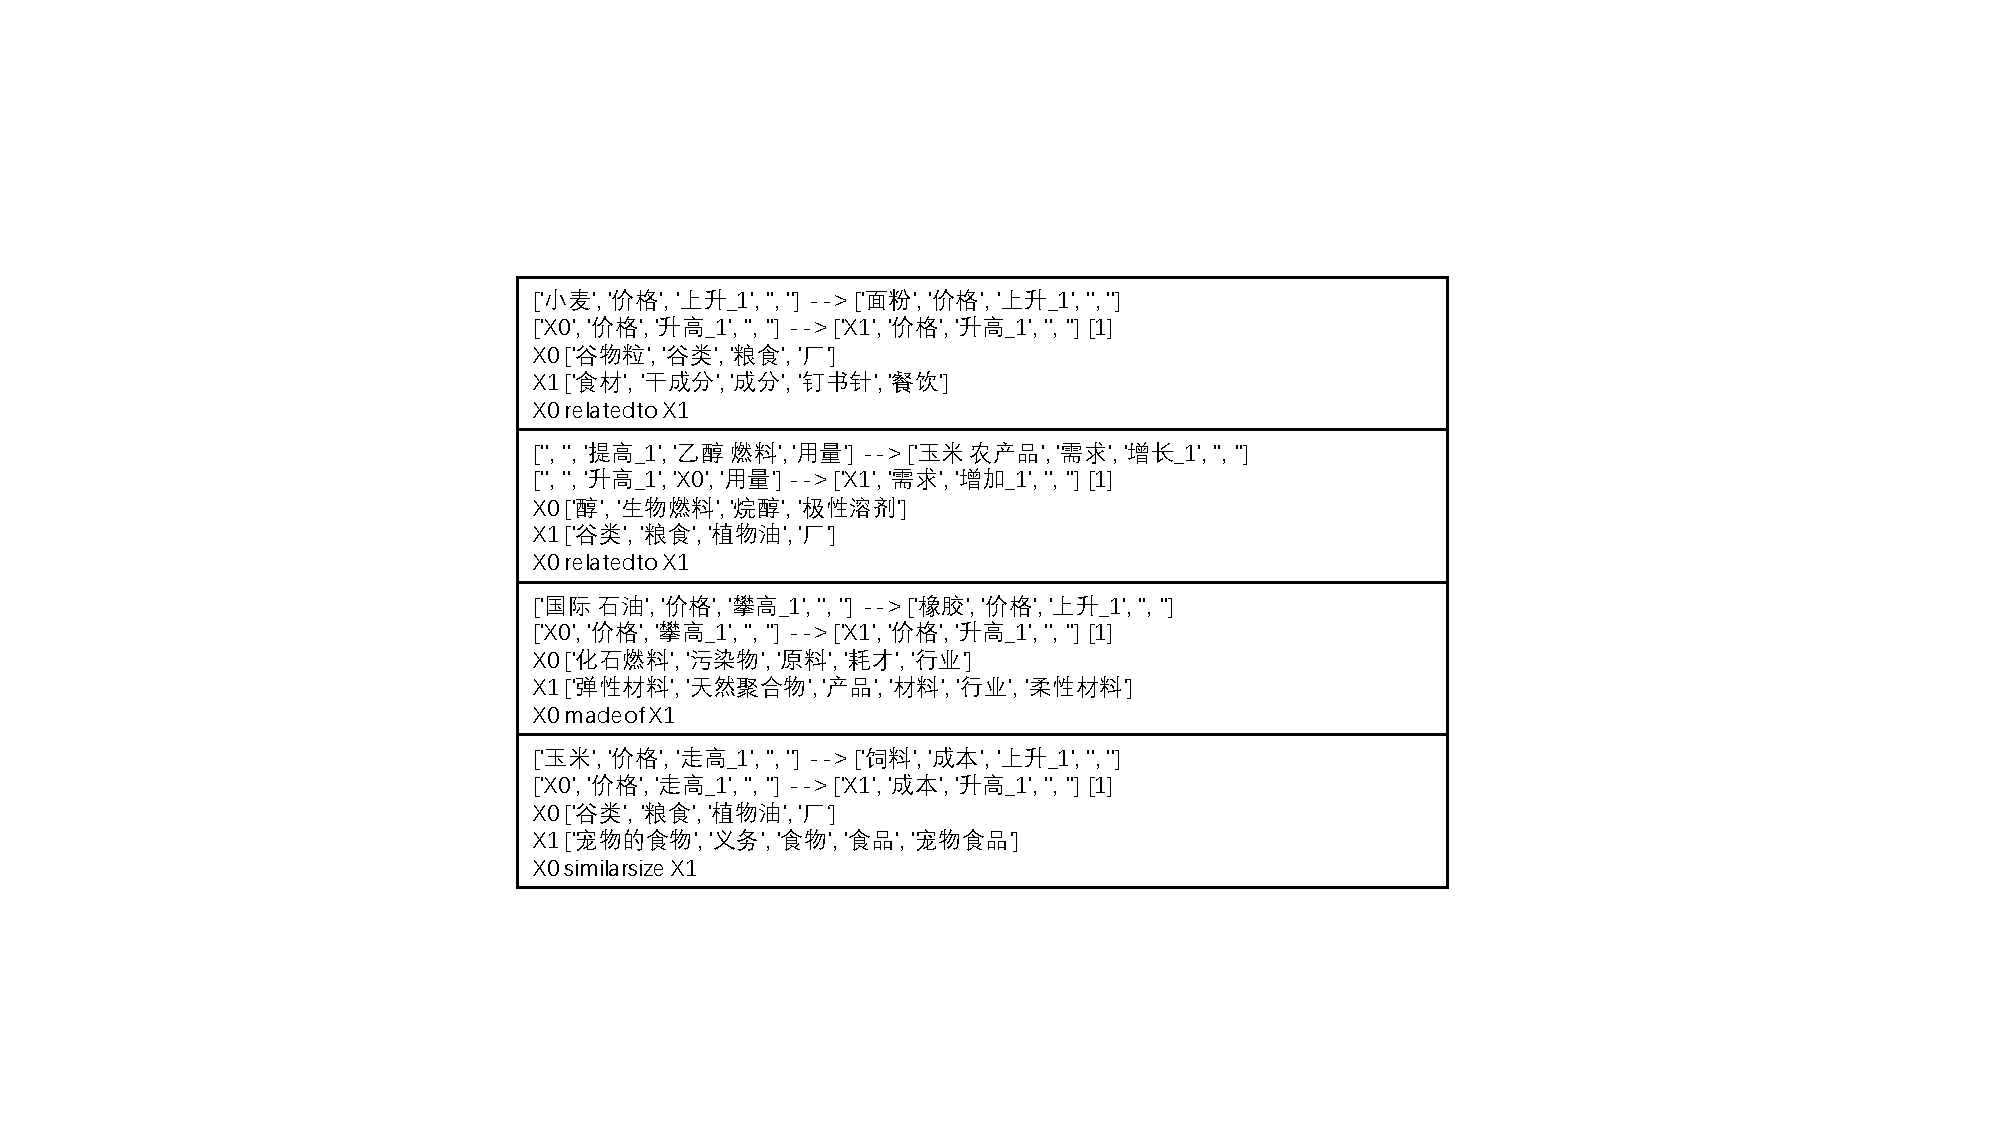
\includegraphics[width=0.95\columnwidth]{figures/reasonable_rule_case}
%	\end{center}
%	\caption{Examples of reasonable Rules.}
%	\label{fig:reasonable_rule_case}
%	\end{figure}
\begin{figure}[htbp]
	\centering
	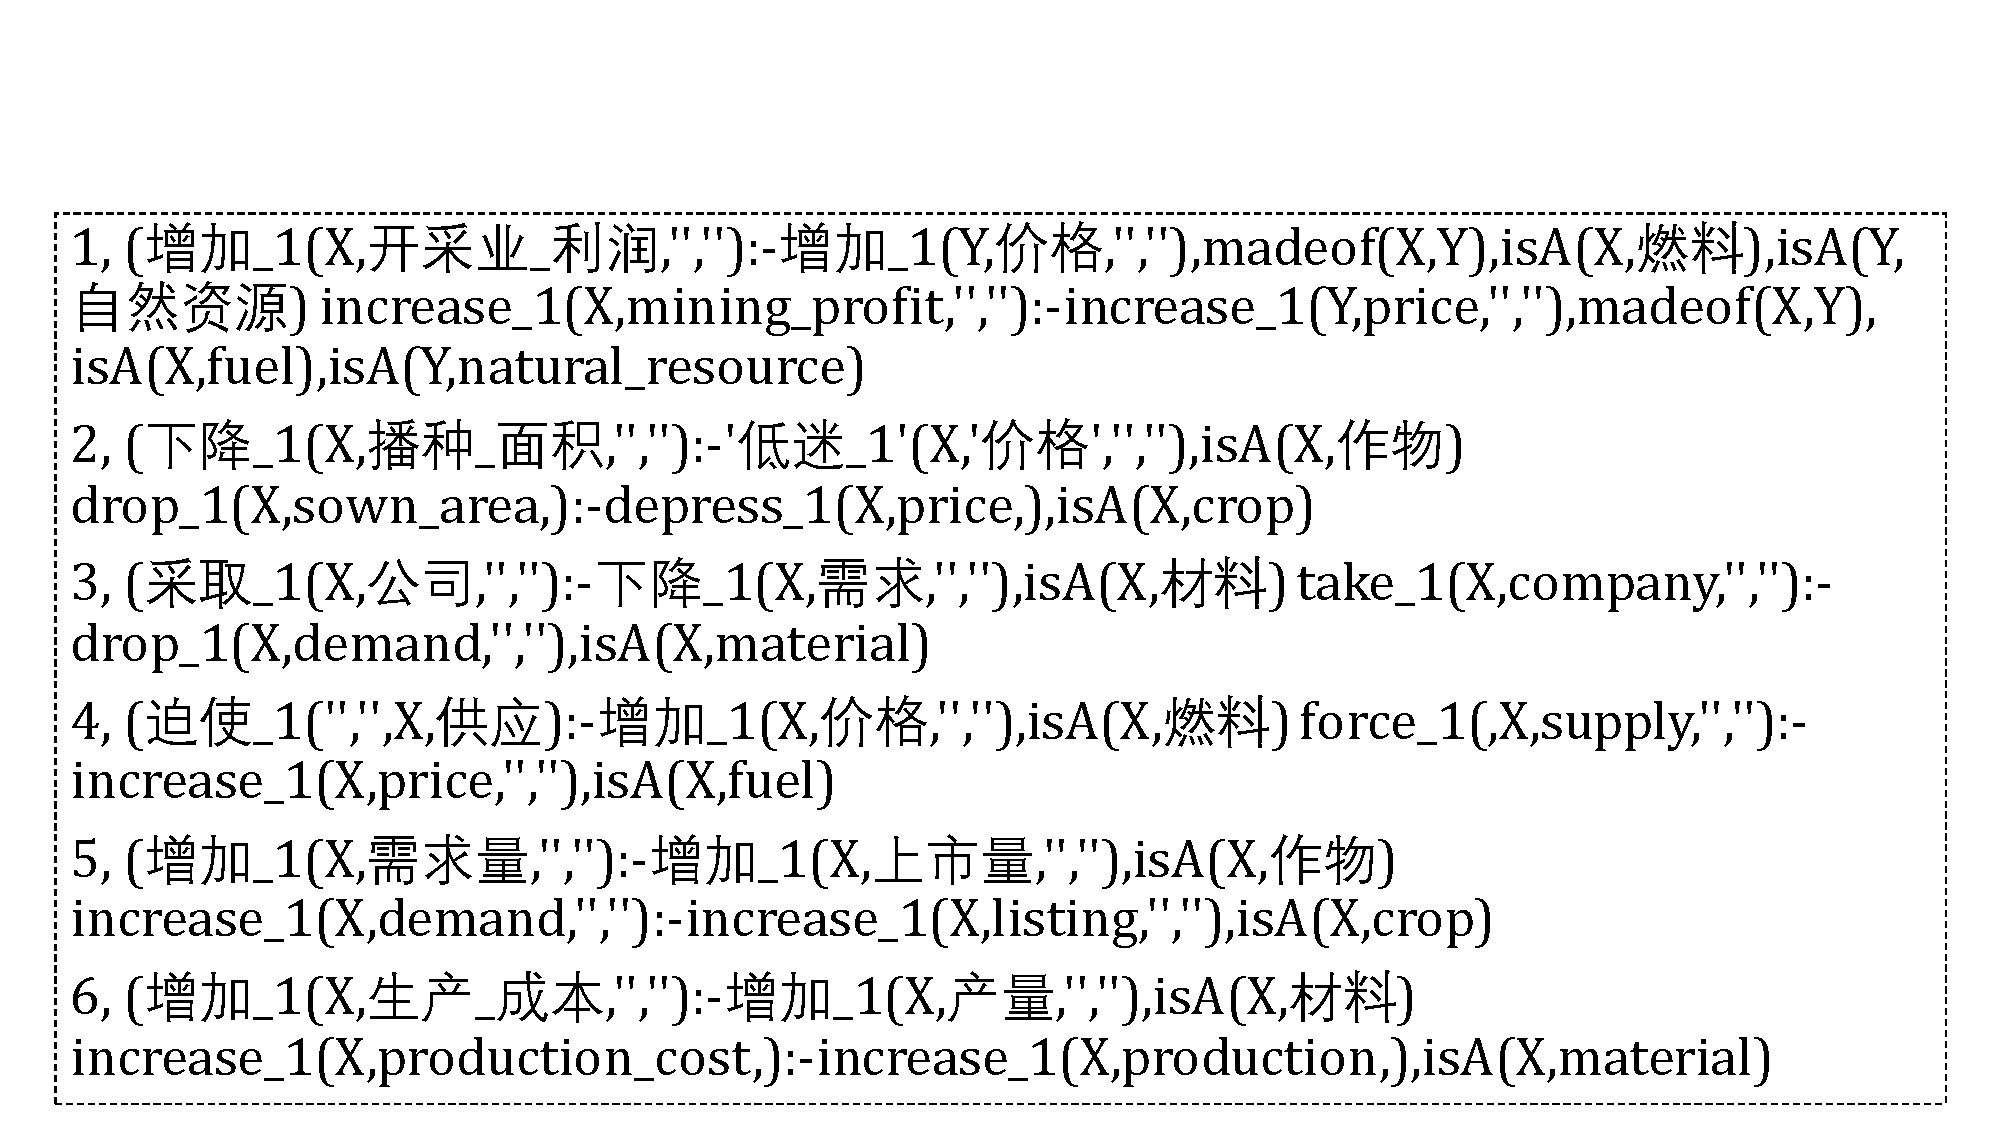
\includegraphics[width=0.95\columnwidth]{figures/rules_case}
	\caption{Examples of Typical Rules}
	\label{fig:rules_case}
\end{figure}
\paragraph{Event Graph}
With these rules, we deduce many rule instances with Prolog and pick out a tiny subgraph about rise and fall events, in Figure\ref{fig:rule_instantiation_graph}, to show the power of the rules. 
	
\begin{figure}[htbp]
\begin{center}
	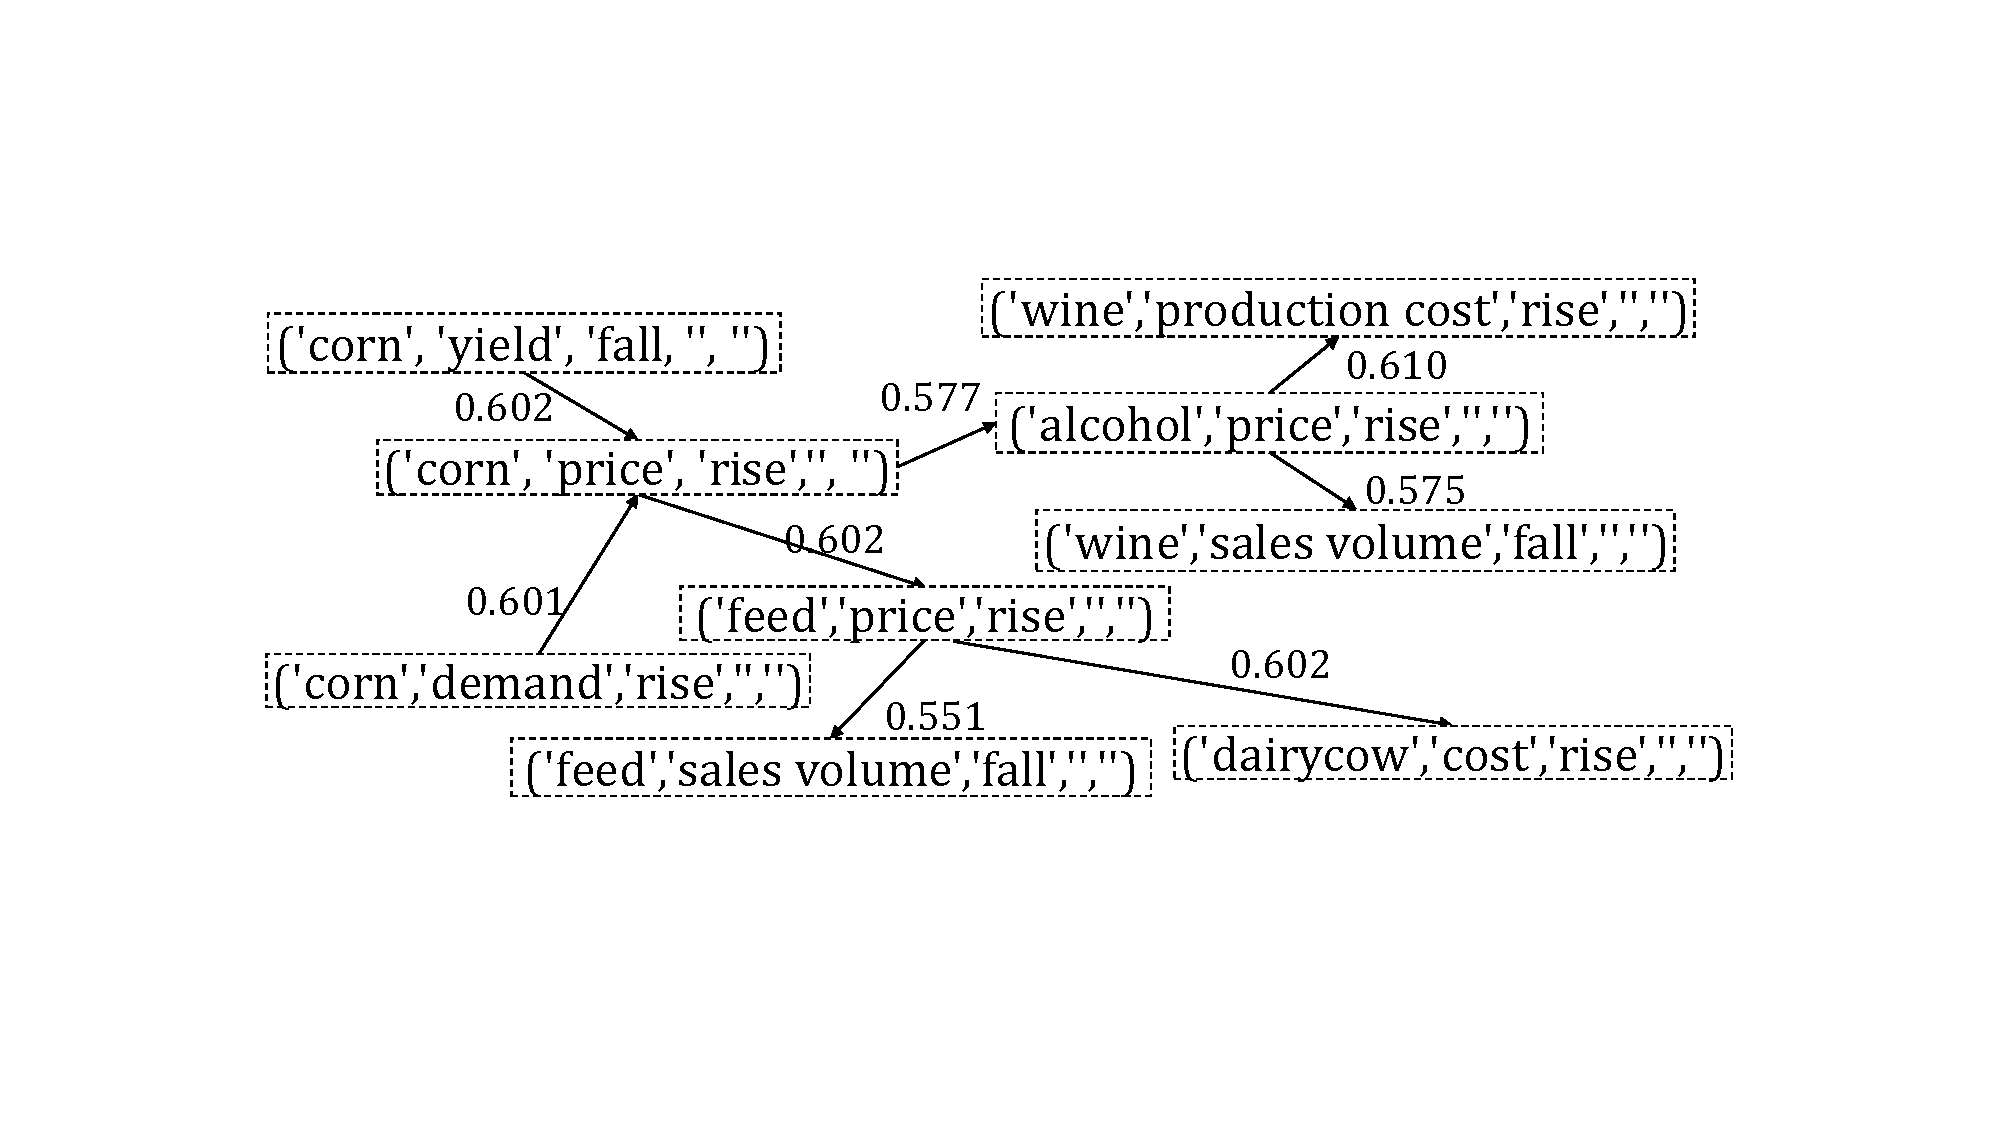
\includegraphics[width=0.9\columnwidth]{figures/instantiation_graph}
\end{center}
\caption{Rule Deduction. As space is limited, we only show the English version and omit the rules used in the reasoning process.}
\label{fig:rule_instantiation_graph}
\end{figure}

\subsection{Comparison with existing Knowledge Bases}
We compare our rules with causal part of other knowledge bases in various aspects in Table \ref{tab:comparison_rule_with_kbs}. We can see our causal knowledge representation is more expressive and informative, and the automatic knowledge acquisition is very convenient.
\begin{table*}[htbp]
\centering
%\begin{tabularx}{\columnwidth}{|c|c|c|c|}\hline
	\begin{tabular}{|c|c|c|c|c|c|c|c|}\hline
	\textbf{Name}&\textbf{Number}&\textbf{Domain}&\textbf{Unit}&\textbf{Data Structure}&\textbf{Information}&\textbf{Source}&\textbf{Precision}\\ \hline
	CausalNet&\textbf{62,675,002}&\textbf{Open}&word&(-)&rich&\textbf{automatic}&-\\
	\multicolumn{8}{|c|}{(`drink',`accident',36)}\\\hline
	ConceptNet &89,416&\textbf{Open}&short text&unstructured&rich&crowdsourcing&\textbf{100\%}\\
	\multicolumn{8}{|c|}{(`smoking',`/r/Causes',`cancer')}\\\hline
	FrameNet&59&\textbf{Open}&frame&\textbf{structured}&richer&crowdsourcing&\textbf{100\%}\\
	\multicolumn{8}{|c|}{Killing(Killer,Place,Means,Victim,Instrument),CausativeOf,Death(Protagonist,Place,Manner,Time)}\\\hline
	ATOMIC&568,312&\textbf{Open}&\textbf{logic event}&semi-structured&much richer&crowdsourcing&86.2\%\\
	\multicolumn{8}{|c|}{If ``PersonX pays PersonY a compliment", Then ``PersonY will smile"}\\\hline
	Ours&50,000&Finance&\textbf{logic event}&\textbf{structured}&\textbf{richest}&\textbf{automatic}&32.5\%\\ 
%			Deductive Rule Instance&\TD{??}\\ 
%	\multicolumn{8}{|c|}{See above rule example in Figure\ref{fig:rules_case}}\\\hline
\multicolumn{8}{|c|}{(Z,`price',`rise',`',`'):-(`',X,`suffer',Y,`attack'),isA(X,`country'),isA(Y,`disaster'),isA(Z,`metal'),atLocation(Z,X) conf:0.842}\\\hline	
	\end{tabular}
%\end{tabularx}  \cite{sap2018atomic}
\caption{Comparison with existing knowledge bases}
\label{tab:comparison_rule_with_kbs}
\end{table*}



%\begin{table}[htbp]
%	\caption{Rule Instance \& Rule}
%	\begin{center}
%	\begin{tabular}{|r|l|}\hline
%		\multicolumn{1}{|c|}{Name}                  & \multicolumn{1}{c|}{Number} \\\hline
%		\multicolumn{1}{|c|}{Rule Instances}        & \multicolumn{1}{c|}{7835403} \\ \hline
%		\multicolumn{1}{|c|}{Rules}                 & \multicolumn{1}{c|}{69036}  \\ \hline
%		\multicolumn{1}{|c|}{more than on relation} & \multicolumn{1}{c|}{2499(3.6\%)}\\
%		\multicolumn{1}{|c|}{only one relation}     & \multicolumn{1}{c|}{66539(96.4\%)} \\
%		\hline
%		==                                          & 56449(84.8\%)                      \\
%		madeof                                      & 5659(8.5\%)                        \\
%		atlocation                                  & 1835(2.76\%)                       \\
%		partof                                      & 1061(1.59\%)                       \\
%		usedfor                                     & 954(1.43\%)                        \\
%		hasa                                        & 511(0.768\%)                       \\
%		derivedfrom                                 & 38(0.0571\%)                       \\
%		hasproperty                                 & 20(0.0301\%)                       \\
%		createdby                                   & 12(0.018\%)                        \\ \hline
%	\end{tabular}
%	\label{tab:rule_statistics}
%\end{center}
%\end{table}
	%Rule Instances & 1817014(4337755)\\
	%Candidate Rules & 86218(201359)\\
	%Rule & 18348(42246)\\

\subsection{Ablation Study}
In this section, we explore the contributions of the various components of our rule learning framework.
\paragraph{Causal patterns statistic} The matched sentences distribution over 3 groups of patterns is shown in Table \ref{tab:pattern_statistics}. All patterns in one group have different causal cue words literally but the same meaning. It shows the third pattern group is more rigorous than the first two groups but has lower usage. Probably because more logical thinking is needed when editing news using more rigorous patterns.

%		\begin{table}[htbp]
%		\caption{Causal patterns. A is a cause tokens span, and B is an effect tokens span. Word '因为' represents a group works like '由于,'是因为','因为','缘于','归因于','原因是','起因','鉴于', and word '所以' represents a group of words like '所以','因而','因此','故此','故而','因故','导致','招致','以致','引致','诱致','致使','造成','使得','从而','从而使','于是','为此'}
%		\begin{center}
%			\begin{tabular}{|c|c|} \hline
%				\textbf{Pattern}& \textbf{Priority}\\ \hline
%				因为 A, 所以B&1\\ \hline
%				A,所以 B&2\\ \hline
%				因为 A,B&3\\ \hline
%			\end{tabular}
%			\label{tab:causal_pattern}
%		\end{center}
%	\end{table}	
	
\begin{table}[htbp]
	\centering
	\begin{tabular}{|c|c|c|c|} \hline
		\textbf{Pattern template}& \textbf{Priority}&\textbf{Number}& \textbf{Rate}\\	\hline 
		因为 A,B&1&2000242&48.32\% \\ \hline 
		A,所以 B&2&1530311&36.96\% \\ \hline 
		因为 A, 所以B&3&576851&14.72\% \\	\hline
	\end{tabular}
	\caption{Number of sentences extracted by causal patterns. A is a cause span and B is an effect span. Word `因为' represents a group works like 由于,是因为,因为,缘于,归因于,原因是,鉴于, and word `所以' represents a group of words like 所以,因而,因此,故而,因故,导致,招致,以致,引致,诱致,致使,造成,使得,从而使,于是,为此}
	\label{tab:pattern_statistics}
\end{table}	
\paragraph{External Knowledge Bases}
The following is some statistics of external knowledge bases used in the rule learning framework. The size of the lexicon is 12,624, obtained from `Industrial classification for national economic activities'\footnote{\url{ http://www.stats.gov.cn/Tjsj/tjbz/hyflbz/}}, which determines which event role in the rule instance can be generalized. 
To our knowledge, most existing Chinese taxonomic knowledge bases, such as CN-Probase\cite{Xu2017}, zhishi.me\cite{Niu2011}, are constructed from online-encyclopedia, which suffer that the concepts inside are far less than Probase and they have no probabilistic character. So we translate Probase to get 11,292,493 Chinese `IsA' pairs.
To our knowledge, there exists no large-scale Chinese commonsense knowledge base, so we translate the English part of ConceptNet and merge the Chinese part to get 2,085,681 Chinese triples.
We randomly sample 500 items from translated Probase and ConceptNet, respectively, and the accuracies after the human evaluation are \textbf{87.8\%}(close to the accuracy of original Probase 92.6\%) and \textbf{91.6\%}.

%\begin{table}[htbp]
%	\centering
%	\begin{tabular}{|c|c|}\hline
%		\textbf{Name}&\textbf{Number}\\ \hline
%		Lexicon&12624\\ \hline
%		Translated Probase &11,292,493(87.8\%)\\ \hline
%		Translated ConceptNet&2,085,681(91.6\%)\\ \hline
%	\end{tabular}
%	\caption{External Knowledge Bases}
%	\label{tab:knowledge_base_statistics}
%\end{table}

%After translation, the number of Chinese IsA pairs is 11,292,493. The number of Chinese commonsense triples is 2,085,681. We both randomly sample 500 items from them, and the accuracy after human evaluation are 0.878 and 0.916 respectively.
%The accuracy of original Probase is 0.926. 
%The number of total Chinese IsA pairs are 11,292,493 which contain concept-instance pairs and concept-subconcept pairs, the. The number of Chinese concepts is 81082 concluding concepts and subconcepts. The number of instances is 158693. The number of Chinese commonsense pairs is 7316977.
%\subsection{External Factual Knowledge Bases}

%From above rule instance extraction submodule, we scan get a rule instances repository. With such huge specific rule instances, we hope to further discover the powerful knowledge hidden in these rule instances. 

%so we generalize such a large amount of rule instances with a more general form. As discussed in Section \ref{sec:intro}, we need to build such a knowledge base. Taxonomy and common sense are two major kinds of knowledge in such knowledge base.
%In our framework, we need to rely on the external Chinese knowledge bases, Chinese Probase and Chinese Conceptnet, to generalize rule instances and add constraints. Most existing Chinese taxonomy knowledge is constructed from online-encyclopedia, such as CN-Probase\cite{Xu2017}. They usually focus more on named entity such as famous movie stars, singer stars, while we care more about the concrete things existed in life such as corn, steel, alcohol and so on.  In addition, they have no probabilistic character. Translation is an effective and efficient approach, we choose to translate Probase, which is a probabilistic taxonomic knowledge base.
%To our knowledge, there exists no large-scale Chinese commonsense knowledge base, so we translate the English part of ConceptNet5 into Chinese and combine the Chinese part.

%	 which is special for this, But it is only for English. We have investigated the CN-Probase\cite{xu2017cn}, but It even can't find the concept of common entities like '中国/China', '橡胶/rubber' and it also limits the usage frequency. So we collect the items from Probase, the items with 'IsA' relation in ConceptNet5\cite{speer2013conceptnet}, Webbrain\cite{chen2016webbrain}. Then, we fuse them together, Then, translate them into Chinese with google translator. to reduce the translate error, we put more context into the translator as more as possible, for example we put 'fruit such as apple, banana', Then we can get the translated result of IsA(apple,fruit), IsA(banana, fruit) together, which can make word sense of 'apple' to be translated near the fruit not company.  
%	\subsubsection{Chinese Commonsense knowledge base.}
%	, consisting of 47, 3, 25 relations respectively. Some of them are duplicative and some are useless for us. So we select specific number useful relations and we also design some patterns to extract some relations from Chinese wiki. 
%	relattions between arguments are used in rule specialization submodule to make rules reasonable. There exist many commonsense knowledge bases such as ConceptNet5, WebBrain, WebChild.  The numbers of the relations in these knowledge bases are limited. And some relations are equivalent among different knowledge bases, such as '/r/RelateTo' in ConceptNet is equivalent to 'relateto' in WebBrain. So we normalize all the relations names literally.
% Meanwhile, many pairs of arguments have more than one relations which are  duplicated semantically. For example, (sweet corn, corn) has the relations 'relatedto' and 'partof', obviously, 'partof' consists of 'relatedto' semantically. So we hope to remove the semantic reduplication relations. which means we need find the semantic containment relations among these relations.
%Algorithm \ref{alg:alg1} shows the Relations Containment algorithm we proposed. It firstly counts each relation and its corresponding arguments pairs. Then, compare the every two correlated relations, and record their containment relation. Last, enumerate all relations in each pair of arguments, remove the relation which is not contained in other relations existed in this pair of arguments.
%When fusing these knowledge bases, we regard arguments from different knowledge bases which have the same literal name as the same arguments.
%	from structured information to knowledge which is close to intelligence
%The goal of rule acquisition is to learn first-order logic rule from huge number of rule instances with the support of external factual knowledge, shown in the Figure \ref{fig:overview}'s middle part.
%with the knowledge base, now, we can generalize the rule instances extracted from rule instances extraction submodule into candidate rules to represent more general knowledge. For example, we hopefully generalize from each cluster of rule instances to one candidate rule. For example, given two rule instances in one cluster, ('国际 石油', '价格', '攀高@攀高', '', '') $->$ ('橡胶', '价格', '上升@升高', '', '') and ('国际 柴油', '价格', '攀高@攀高', '', '') $->$ ('橡胶', '价格', '上升@升高', '', ''), the generalized candidate rule would be('X0', '价格', '攀高', '', '') $->$ ('X1', '价格', '升高', '', '') where 'X0' IsA' 化石燃料','原料' and  'X1' IsA '弹性材料' '天然聚合物'.


%\begin{table}[htbp]
%\centering
%		\begin{tabular}{|c|c|}\hline
%			\textbf{Name}&\textbf{Number}\\ \hline
%			Lexicon&12624\\ \hline
%			Concepts &18281\\	
%			IsA pairs &123547\\
%			Concept-subconcept pairs&18753\\
%			Concept-instance pairs&104794\\\hline
%			Commonsense Pairs&32593\\ 
%			Commonsense Relations&10\\ \hline
%		\end{tabular}
%		\caption{Knowledge Base}
%		\label{tab:knowledge_base_statistics}
%\end{table}
\paragraph{Open Event Extraction}
%	TextRunner/WOE,ReVerb,Ollie,ClausIE,SRL/AMR parsing/frame-semantic parsing,NestIE 
Since our event structure scheme is plain and straightforward, we choose the reliable Stanford CoreNLP tool to extract the rule instances.
%	rule instance  97/200(48.5\%)& 21/200(10.5\%) & 82/200(41.0\%) \\ \hline
The number of rule instances extracted after rule instance distilling submodule is 7,835,403. Since most of them are discarded in the learning process, the number of rule instances really used for rule induction is 78,098 with an accuracy of \textbf{48.5\%} (we also sample 200 rule instances and manually evaluate them).

%\textit{To sum up}, our framework is a pipeline, in which rule instance extraction achieve 48.5\%, ConceptNet5 translation achieve 91.6\% and Probase translation achieves 87.8\%, So teh rule finally can achieve 39.0\%(48.5\%*91.6\%*87.8\%) maximumly, which is close to the evaluation of the final rules. 

%\textbf{\textit{To sum up}}, 
%our framework is a pipeline, in which the accuracy of rule instance extraction is 48.5\%, the accuracy of ConceptNet5 translation is 91.6\%, and the accuracy of Probase translation is 87.8\%. 
\textbf{\textit{To sum up}}, our framework is a pipeline undergoing rule instance extraction(accuracy 48.5\%), constrain relations addition(accuracy of ConceptNet 91.6\%), and rule induction(accuracy of Probase 87.8\%).
Thus, the accuracy can only reach \textbf{39.0\%} (48.5\%*91.6\%*87.8\%) at the maximum, which is close to our evaluation(32.5\%) of the final rules.

%	\subsubsection{Rule Acquisition}
%	\begin{table}[]
%		\centering
%		\begin{tabular}{lll}
%			& rule number  & qualitity       \\
%			no Coneptnet / only one relation    & 66539/96.4\% & informative     \\
%			Conceptnet / more than one relation & 2499/3.6\%   & more infrmative
%		\end{tabular}
%		\caption{Relation Number}
%	\end{table}

%	\begin{table}[]
%		\caption{Event Connection}
%		\begin{center}
%		\begin{tabular}{lll}
%			==         & 60475 & 84.4\%  \\
%			madeof     & 6161  & 8.6\%   \\
%			atlocation & 2104  & 2.94\%  \\
%			partof     & 1152  & 1.61\%  \\
%			usedfor    & 1072  & 1.5\%   \\
%			others     & 674   & 0.941\%
%		\end{tabular}
%		\end{center}
%	\end{table}
\subsection{Application: Futures Price Prediction}
%\paragraph{Reasoning with Uncertainty}
\begin{figure}[htbp]
	\begin{center}
		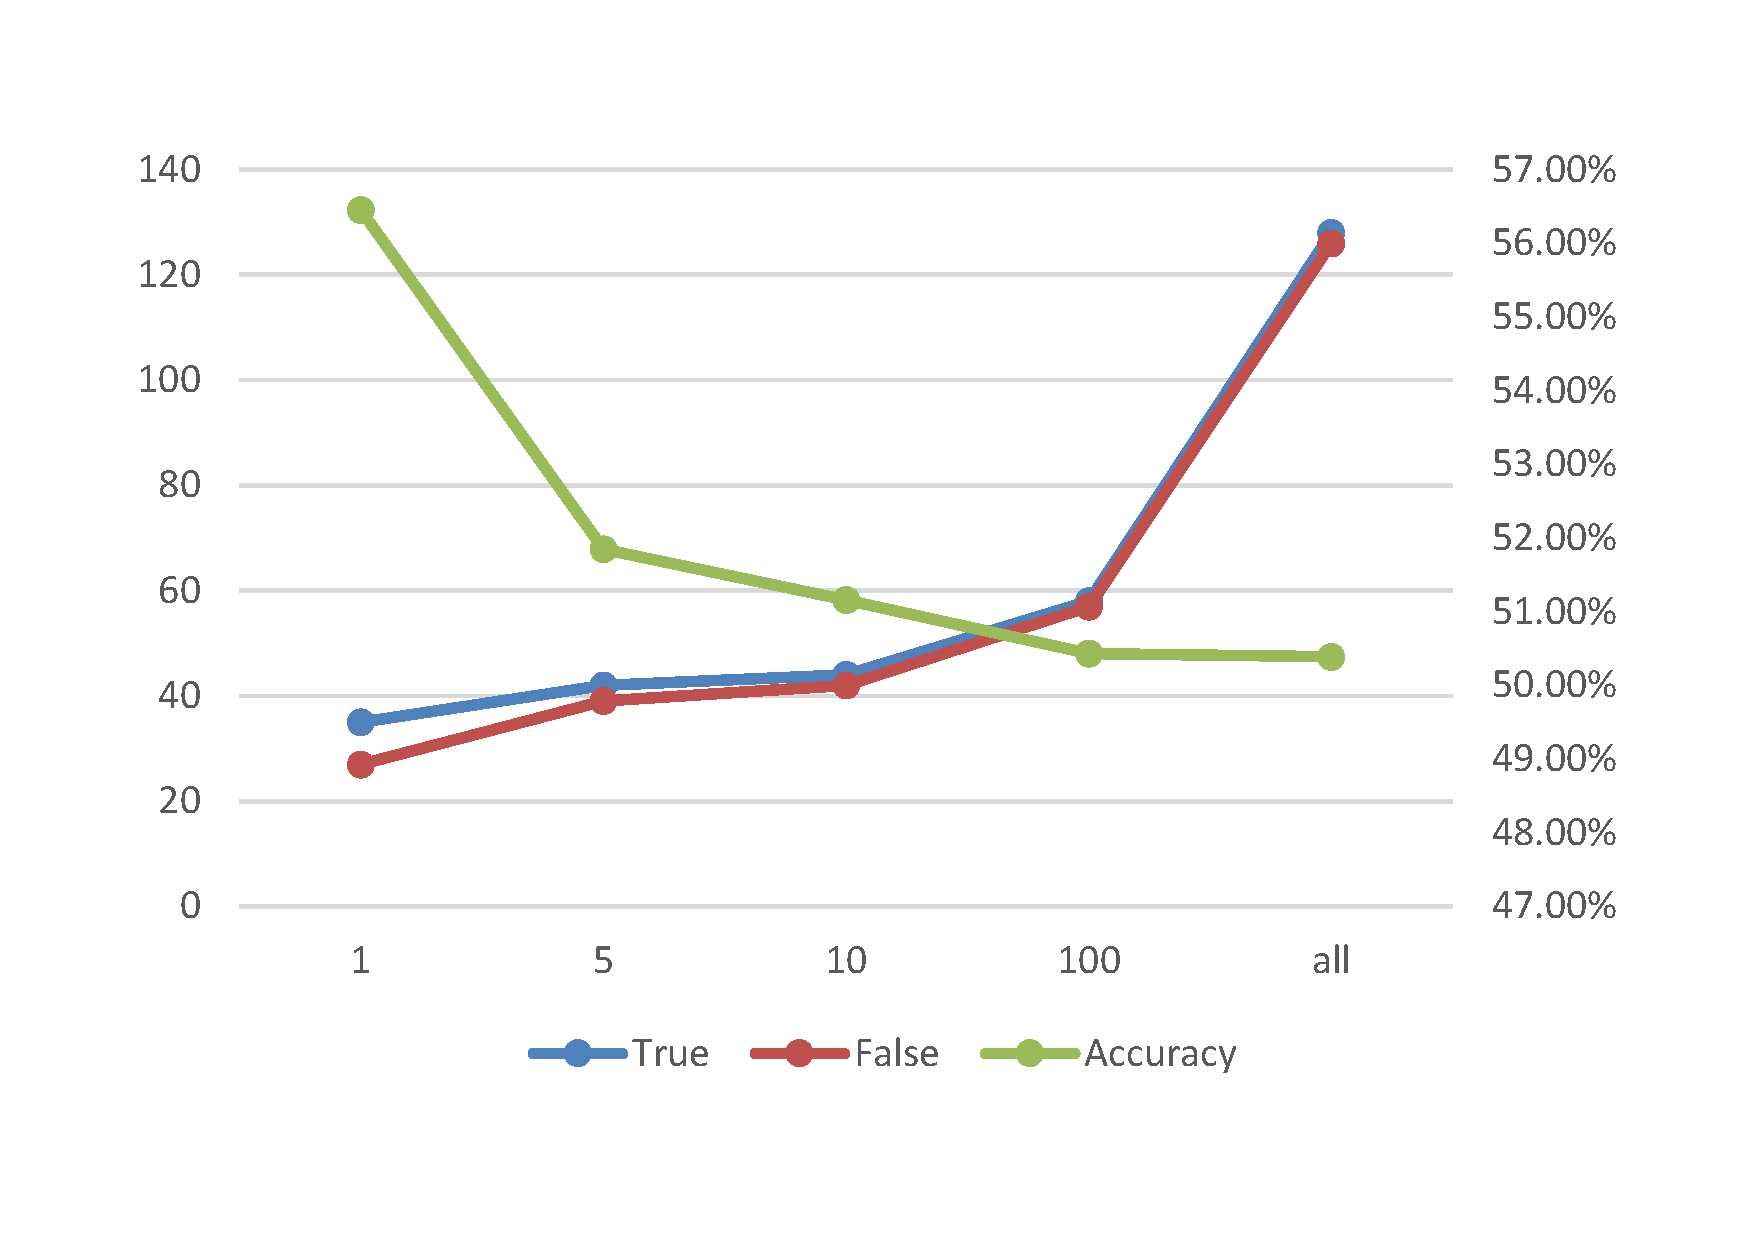
\includegraphics[width=0.9\columnwidth]{figures/rule_futures_prediction}
	\end{center}
	\caption{Futures Price Prediction.}
	\label{fig:futures_price_prediction}
\end{figure}
We choose futures price prediction because the futures are common and concrete things existed in ConceptNet and Probase, such as corn, oil, etc.
%\cite{Ding} is the state-of-the-art stock prediction model(EB\_CNN). We follow similar experimental settings. 
We follow similar experimental settings in \cite{Ding}.
From 2018/1/1 to 2018/11/2, we collect all the headlines and the price change of 15 futures as test data, which include \textbf{851} price change events (The price change of more than 1\% relative to the previous day is an event and we only focus on rise or fall events). 

Baseline models: EB\_CNN model \cite{Ding}, the state of the art model in stock price prediction, uses a deep convolutional neural network to model both short-term and long-term influences of events on stock price movements, and the accuracy of futures prediction is \textbf{54.2\%}. Other models in \cite{Ding}, such as EB\_NN, WB\_CNN, and WB\_NN can achieve \textbf{53.0\%}, \textbf{53.2\%}, and \textbf{53.5\%}, respectively. These accuracies of futures prediction are lower than the accuracies of stock prediction shown in the paper.
It may be because the factors affecting the futures price are far less than the stock price and the futures price is much more stable than the stock price, which makes useful training information about the futures less and further affects the accuracy of the models.

Our approach: For each actual future price change event , we get the news headlines for the previous month before this event. 
For each news headline, we extract the event, use Prolog to reason based on the rules and external knowledge bases, and get the top K inferred events sorted by the confidence.
We may have m*K inferred events for this event, m is the number of events occurred in this month. 
Here, we select the price change events(rise or fall) of the future in this actual future price change event from m*K events and calculate the weighted sum of their confidences(rise event weights 1 and fall event weights -1). If the sum value is positive, we predict this future price as a rise event, otherwise as a fall event. If get no related events changing the future's price, do not make prediction. We compare this prediction with the actual price change to evaluate the reasoning effect. 
Figure \ref{fig:futures_price_prediction} shows the average prediction result. It shows the more predicted events inferred from the Prolog(by increasing K) we use, the lower the prediction accuracy is(from \textbf{56.5\%} to \textbf{50.4\%}), and the more futures events we can predict(from \textbf{62} to \textbf{254}). 

\textbf{\textit{To sum up}}, our rule-based prediction approach can have a higher prediction accuracy (56.45\%) and better interpretation ability with a low recall rate, which is very practical in life.

%\begin{table}[htbp]
%	\caption{Baselines and Proposed Framework}
%	\begin{center}
%		\begin{tabular}{lll}\hline
%			& Acc & MCC \\\hline
%			WB-NN &  0.535 &     \\
%			WB-CNN&  0.532  &     \\
%			EB-NN &  0.530  &     \\
%			EB-CNN&  0.542   &     \\
%			Rule &     &    \\\hline
%		\end{tabular}
%		\label{tab:baselines_and_rule}
%	\end{center}
%\end{table}

\subsection{Downloading and Demo}
The translated Chinese Probase and ConceptNet and learned rules are available at URL.
We built a demo to demonstrate the reasoning process at URL. 
We also developed an application demo of futures prices change triggering that can monitor news from around the world in real time, find the news that may cause futures prices changes, and alert users. Visit URL.
\section{Conclusion}

In this paper, we incorporated the idea of Cookie Theft picture description task into the evaluation of the high-level cognitive abilities of LVLMs and designed a novel evaluation benchmark called CogBench.
% Images in CogBench are of high quality and require more cognitive reasonings to understand, which makes it different from existing image datasets.
The images in CogBench are of high quality and demand more complex cognitive reasoning for interpretation, setting it apart from existing image datasets.
% It consists of a image description task and a VQA task.
Experiments show that there is still a large gap between the cognitive abilities of LVLMs and human beings, indicating CogBench is a challenging benchmark.

% In the future

\section{Ethical Statement}
\label{sec:ethics}

Our study adheres to the ethical requirements in place, and we make every effort to protect the privacy and respect the willingness of our participants.

During participant recruitment, we required patients to read and sign an informed consent form. This ensured that they understood the objectives of the entire project, the research content, potential risks and benefits, and the purpose of data collection. Only after their agreement and signature were obtained, the evaluation process officially commenced. We also assured them that they could voluntarily withdraw from the study at any stage.

In order to safeguard the privacy of our participants, we took measures to anonymize the collected dialogue history. This was done by replacing usernames with random identifiers, ensuring that any information that could identify individuals was excluded from our research process. Additionally, we conducted thorough manual filtering of the dialogue histories to eliminate any offensive content or language that may encourage self-harm or suicide.


\section*{Limitations}
\label{sec:limitation}

Limitations

% Entries for the entire Anthology, followed by custom entries
\bibliography{anthology,custom}
\bibliographystyle{acl_natbib}

\appendix

\section{Depression Templates}

\begin{table}[htbp]
  \small
  \centering
  \begin{tabular}{l|l}
  \hline
  Dimension & Template \\
  \hline
  Feeling Depressed  &  I feel depressed. \\
  Diagnosis &  I am diagnosed with depression. \\
  Treatment &  I am treating my depression. \\
  \hline
  Sadness & I feel sad.  \\
  Pessimism & I am discouraged about my future.  \\
  Past Failure & I always fail. \\
  Loss of Pleasure & I don't get pleasure from things. \\
  Guilty Feelings & I feel quite guilty. \\
  Punishment Feelings & I expected to be punished. \\
  Self-Dislike & I am disappointed in myself. \\
  Self-Criticalness & I always criticize myself for my faults. \\
  Suicidal Thoughts or Wishes & I have thoughts of killing myself. \\
  Crying & I always cry. \\
  Agitation & I am hard to stay still. \\
  Loss of Interest & It's hard to get interested in things. \\
  Indecisiveness & I have trouble making decisions. \\
  Worthlessness & I feel worthless. \\
  Loss of Energy & I don't have energy to do things. \\
  Changes in Sleeping Pattern & I have changes in my sleeping pattern. \\
  Irritability & I am always irritable. \\
  Changes in Appetite & I have changes in my appetite. \\
  Concentration Difficulty & I feel hard to concentrate on things. \\
  Tiredness  & I am too tired to do things. \\
  Loss of Interest in Sex & I have lost my interest in sex. \\
  \hline
  \end{tabular}
  \caption{The main templates and their corresponding dimensions we used in our experiments, including 3 direct depression descriptions and 21 indirect symptoms derived from BDI-II \citep{beck1996beck}. }
  \label{table:bdi}
\end{table}


We provide the complete templates in Table \ref{table:bdi}. We mainly use a combination of 3 direct depression descriptions and the 21 indirect symptoms derived from BDI-II. We also experimented other well-known depression scales like HDRS \citep{hamilton1986hamilton}, CES-D \citep{Lenore1977CES-D} and PHQ-9 \citep{kroenke2001phq} (We will release our revised templates for theses scales along with our code). The original scales usually contain different descriptions under the same dimension to distinguish different level of intensity or frequency. However, we find that current sentence representations have difficulty in capturing such nuanced differences. We thus condense the descriptions of each dimension into one general template (A few may have more, if there are significant intra-dimension difference).

\section{Related Work}
\paragraph{Clarification Question Generation} The concept of CQ can be naturally raised in a dialogue system where the speech recognition results tend to be erroneous so that we raise CQs for sanity check \citep{stoyanchev2014towards}, or the intents for a task is incomplete or ambiguous in a first short utterance and further CQs are needed to fill in the slots \citep{dhole2020resolving}. The concept is then extended to IR to clarify ambiguous queries \citep{aliannejadi2019asking}, and has been successfully put into practice \citep{zamani2020generating}. Other application areas including KBQA \citep{xu2019asking} and open-domain dialogue systems \citep{aliannejadi2020convai3}. CQGen can also be applied to help refine posts on websites like StackExchange \citep{Kumar_2020} and Amazon \citep{rao2019answer}. In this context, our work closely follows the research line of \citep{rao2018learning, rao2019answer, cao2019controlling}. \citet{rao2018learning} first adopted a retrieval-then-rank approach. They \citep{rao2019answer} then proposed a generation approach to train the model to maximize the utility of the hypothetical answer for the questions with GAN, to better promote specificity. \citet{cao2019controlling} propose to control the specificity by training on data with explicit indicator of specificity, but it requires additional specificity annotation. Towards the similar specificity goal, we adopted a different keyword-based approach. They also assume generating one question per context, which we claim is not sufficient to cover various possible information needs, and thus propose the task of the diverse CQGen.

\paragraph{Diverse Generation} The demand for diverse generation exists in many other fields~\cite{vijayakumar2018diverse, LiangZ18code, shen2019mixture}, and we've drawn inspirations from these literatures. For image captioning, we may use multiple descriptions for different focusing points of a scene. \textit{Diverse Beam Search} \citep{vijayakumar2018diverse} was proposed to broaden the searching space to catch such diversity by dividing groups in decoding and imposing repetition penalty between them. For machine translation, a context can be translated with different styles. \citet{shen2019mixture} thus proposed \textit{Mixture of Expert} models including hMup to reflect various styles with a discrete latent variable (\textit{expert}). And here for CQGen, diversity is required to cover various potentially missing aspects, so we come up with the idea to use keywords as a controlling variable like \textit{expert} to promote diversity.



\end{document}
